\documentclass[12pt,letterpaper]{article}

\usepackage[spanish]{babel}
\usepackage[utf8]{inputenc}
\usepackage[T1]{fontenc}
\usepackage{graphicx}
\usepackage[hidelinks]{hyperref}
\usepackage{float}
\usepackage{geometry}
\usepackage[table]{xcolor}
\usepackage{tabularx}
\usepackage{array}
\usepackage{booktabs}
\usepackage{placeins}
\usepackage{enumitem}
\usepackage{setspace}
\usepackage{parskip}
\usepackage{ragged2e}
\usepackage{caption}
\usepackage{tocloft}
\usepackage{titlesec}
\usepackage{fancyhdr}
\geometry{left=2.5cm,right=2.5cm,top=3.0cm,bottom=2.5cm}
\graphicspath{{../common/assets/}{../layouts/}{../layouts/stitch/}}

\definecolor{gymblue}{HTML}{1565C0}
\definecolor{gymblueDark}{HTML}{0D47A1}
\definecolor{gymblueSoft}{HTML}{E3F2FD}
\definecolor{gymblueSoftAlt}{HTML}{F4F9FF}

\newcolumntype{Y}{>{\raggedright\arraybackslash}X}
\newcolumntype{L}[1]{>{\raggedright\arraybackslash}p{#1}}
\newcommand{\gymtableheaderrow}{\rowcolor{gymblue}}
\newcommand{\gymth}[1]{\textcolor{white}{\textbf{#1}}}
\newcommand{\storycell}[1]{\begin{minipage}[t]{\linewidth}\vspace{2pt}#1\vspace{2pt}\end{minipage}}
\newcommand{\storyitems}[1]{\storycell{\begin{enumerate}[leftmargin=1.4em,itemsep=2pt,topsep=2pt,parsep=0pt,partopsep=0pt]#1\end{enumerate}}}
\renewcommand{\arraystretch}{1.25}
\renewcommand{\cftsecleader}{\cftdotfill{\cftdotsep}}
\renewcommand{\cftsubsecleader}{\cftdotfill{\cftdotsep}}
\addto\captionsspanish{
  \renewcommand{\contentsname}{ÍNDICE GENERAL}
  \renewcommand{\listfigurename}{ÍNDICE DE FIGURAS}
  \renewcommand{\listtablename}{ÍNDICE DE TABLAS}
}
\setlength{\cftbeforetoctitleskip}{0pt}
\setlength{\cftaftertoctitleskip}{12pt}
\renewcommand{\cfttoctitlefont}{\fontsize{12}{14}\selectfont\bfseries}

\titleformat{\section}{\fontsize{12}{14}\selectfont\bfseries\centering}{\thesection.}{0.5em}{\MakeUppercase}
\titlespacing*{\section}{0pt}{6pt}{6pt}
\titleformat{\subsection}{\fontsize{12}{14}\selectfont\bfseries}{\thesubsection}{0.5em}{}
\titlespacing*{\subsection}{0pt}{6pt}{6pt}
\titleformat{\subsubsection}{\fontsize{11}{13}\selectfont\bfseries}{\thesubsubsection}{0.5em}{}
\titlespacing*{\subsubsection}{0pt}{6pt}{6pt}

\pagestyle{fancy}
\fancyhf{}
\fancyhead[L]{\textcolor{gymblueDark}{\textbf{GymFlow}}}
\fancyhead[R]{\textcolor{gymblueDark}{Informe final del proyecto}}
\fancyfoot[C]{\thepage}
\setlength{\headheight}{25pt}
\renewcommand{\headrulewidth}{0.6pt}
\renewcommand{\headrule}{\hbox to\headwidth{\color{gymblue}\leaders\hrule height \headrulewidth\hfill}}
\setlength{\parindent}{0pt}
\AtBeginDocument{\singlespacing\setlength{\parskip}{6pt}\justifying}

\begin{document}
\begin{titlepage}
\centering
\vspace*{0cm}
\begin{minipage}[c]{0.18\textwidth}
  \centering
  
\includegraphics[width=0.8\textwidth]{../common/assets/logo_left.png}
\end{minipage}%
\hfill
\begin{minipage}[c]{0.64\textwidth}
  \centering
  {\fontsize{12}{15}\selectfont\bfseries
  UNIVERSIDAD MAYOR DE SAN SIMÓN\\[4pt]
  FACULTAD DE CIENCIAS Y TECNOLOGÍA\\[4pt]
  CARRERA DE INGENIERÍA INFORMÁTICA}
\end{minipage}%
\hfill
\begin{minipage}[c]{0.18\textwidth}
  \centering
  
\includegraphics[width=0.9\textwidth]{../common/assets/logo_right.png}
\end{minipage}

\vspace{2.3cm}

{\fontsize{16}{28}\selectfont\bfseries GYMFLOW}\\[0.25cm]
{\fontsize{14}{20}\selectfont\bfseries INFORME FINAL DEL PROYECTO}\\[0.45cm]

{\large{Sistema Inteligente de Entrenamiento por Músculos}}\\[0.3cm]

\vspace{0.5cm}

\setstretch{1.4}
{\large
\textbf{Materia:} Programación Móvil\\[8pt]
\textbf{Docente:} Dr. Américo Fiorilo Lozada Ph.D.\\[8pt]
\textbf{Carrera:} Ingeniería Informática\\[10pt]
\textbf{Integrantes del grupo y roles:}
}

\vspace{6pt}

{\normalsize
\begin{tabular}{@{}ll@{}}
Chamaca Jimenez Cristhian & Desarrollador Full Stack \\[3pt]
Montaño Frías Andres & Desarrollador Full Stack \\[3pt]
Mita Zeballos Cristian Juan & Scrum Master \\[3pt]
Zeballos Valencia Reynaldo & Desarrollador Full Stack \\
\end{tabular}
}

\vspace{12pt}

{\large \textbf{Fecha de presentación:} 8 de junio de 2026}

\vfill

{\large\bfseries COCHABAMBA -- BOLIVIA}\\[4pt]
{\normalsize Junio -- 2026}

\end{titlepage}

\clearpage
\tableofcontents
\clearpage

\section{Resumen Ejecutivo}

GymFlow es una aplicación móvil orientada a apoyar al usuario durante su sesión de entrenamiento en el gimnasio. Su propósito principal es permitir la consulta rápida de grupos musculares, ejercicios y variantes útiles cuando una máquina o implemento no se encuentra disponible, reduciendo así la improvisación y mejorando la continuidad de la rutina.

El proyecto se desarrolla con React Native y Expo, utilizando servicios de Firebase para autenticación y almacenamiento de información. El presente documento constituye el \textbf{informe final del proyecto} y reúne, en un solo documento, el análisis del problema, el diseño de la solución, la arquitectura del sistema, la metodología de desarrollo, la planificación, las pruebas y las conclusiones.

A diferencia de cortes anteriores limitados a la fase de acceso, esta versión refleja el \textbf{sistema efectivamente implementado}, que abarca la autenticación con correo y con Google, la configuración personalizada del perfil mediante un onboarding guiado, la consulta de músculos, ejercicios y variantes, la creación y gestión completa de rutinas, la planificación y ejecución de las sesiones de entrenamiento (con registro de series, peso, repeticiones y RPE), el historial detallado y el funcionamiento sin conexión. La trazabilidad de estas funcionalidades se documenta mediante las historias de usuario HU-01 a HU-26.

\section{Análisis del Proyecto}

\subsection{Objetivo general}

Desarrollar una aplicación móvil denominada \textbf{GymFlow} que permita a los usuarios seleccionar los músculos que desean entrenar y visualizar diferentes ejercicios y variantes para optimizar sus rutinas de entrenamiento dentro del gimnasio.

\subsection{Objetivos específicos}

\begin{itemize}
    \item Implementar un sistema de registro e inicio de sesión para los usuarios de la aplicación.
    \item Mostrar los principales grupos musculares que pueden ser entrenados dentro del gimnasio.
    \item Proporcionar ejercicios asociados a cada grupo muscular.
    \item Sugerir variantes de ejercicios que permitan entrenar el mismo músculo cuando una máquina se encuentre ocupada.
    \item Permitir la creación de rutinas de entrenamiento personalizadas.
    \item Permitir guardar y consultar rutinas de entrenamiento creadas por el usuario.
    \item Ofrecer rutinas prediseñadas para facilitar el entrenamiento de los usuarios.
    \item Implementar un módulo de administración que permita gestionar ejercicios, músculos y rutinas prediseñadas.
    \item Registrar el historial de entrenamientos realizados por el usuario.
\end{itemize}

\subsection{Problemas identificados}

\subsubsection{Situación problemática}

Dentro del entorno del gimnasio, los usuarios suelen seguir rutinas organizadas por grupos musculares y ejercicios específicos. Estas rutinas, en muchos casos, han sido planificadas previamente con un orden determinado, un número de series y repeticiones, y el uso de máquinas o implementos concretos. Sin embargo, en la práctica, la sesión de entrenamiento no siempre puede desarrollarse tal como fue diseñada.

Uno de los escenarios más frecuentes ocurre cuando el usuario llega a una máquina o equipo determinado y descubre que este se encuentra ocupado. Esta situación es común en horarios de mayor concurrencia, donde varios usuarios coinciden en el uso de los mismos recursos. A partir de ello, la rutina deja de depender únicamente de la planificación personal y pasa a estar condicionada por la disponibilidad real del entorno.

\subsubsection{Problema principal}

El problema principal identificado es la dificultad que tienen los usuarios para continuar su rutina de entrenamiento de manera ordenada y eficiente cuando una máquina o equipo específico no se encuentra disponible.

Esta dificultad no solo representa una molestia momentánea, sino que afecta directamente la continuidad de la sesión. Cuando el usuario no puede ejecutar el ejercicio previsto, debe decidir entre esperar, cambiar el orden de su rutina o sustituir el ejercicio por otro. En ausencia de una guía clara, esta decisión suele tomarse de manera improvisada, lo cual reduce la calidad del entrenamiento y altera la lógica originalmente planificada.

\subsubsection{Factores asociados al problema}

El problema descrito está relacionado con diversos factores propios del entorno y del usuario. En primer lugar, la alta concurrencia en determinados horarios provoca que muchas máquinas y estaciones de trabajo permanezcan ocupadas durante varios minutos. Este factor es propio del funcionamiento normal de los gimnasios y afecta especialmente a los usuarios que dependen de equipos concretos para completar su rutina.

En segundo lugar, existe una dependencia considerable respecto a ejercicios específicos. Aunque varios músculos pueden trabajarse mediante distintas variantes, muchos usuarios estructuran su sesión alrededor de una secuencia fija de ejercicios, sin contemplar desde el inicio posibles alternativas.

En tercer lugar, muchos asistentes al gimnasio no cuentan con el conocimiento suficiente sobre variantes o ejercicios equivalentes. Esta limitación es más notoria en usuarios principiantes, quienes todavía no dominan la relación entre grupo muscular, ejercicio principal y posibles sustituciones. Como resultado, ante un imprevisto, no disponen de criterios claros para adaptar su entrenamiento.

Finalmente, también se observa la ausencia de una herramienta móvil centrada específicamente en esta problemática. Si bien existen aplicaciones de fitness, no todas responden a la necesidad inmediata de consultar músculos, ejercicios y variantes en función de la disponibilidad de equipos dentro del gimnasio.

\subsubsection{Manifestaciones del problema}

A partir del problema principal, se identifican varias situaciones concretas que afectan al usuario durante su sesión de entrenamiento.

Una de ellas es la pérdida de tiempo provocada por la espera de máquinas ocupadas. En lugar de mantener un ritmo constante de trabajo, el usuario interrumpe su actividad y reduce el tiempo efectivo de entrenamiento.

Otra manifestación importante es la modificación improvisada de la rutina. Cuando no existe una referencia clara sobre alternativas, el usuario puede elegir ejercicios sin suficiente criterio técnico, alterando el enfoque muscular originalmente previsto.

También se presenta el desconocimiento de variantes funcionales. Muchos usuarios saben ejecutar un ejercicio específico, pero no necesariamente conocen otras opciones que permitan trabajar el mismo músculo mediante un movimiento similar o con otro tipo de implemento.

Asimismo, algunos ejercicios son omitidos por completo, lo que ocasiona sesiones incompletas o desequilibradas. Esto ocurre cuando el usuario prefiere continuar con otras partes de la rutina antes que buscar una sustitución adecuada.

\subsubsection{Consecuencias para el usuario y el entrenamiento}

Las consecuencias de esta problemática se reflejan tanto en la experiencia del usuario como en la calidad del entrenamiento realizado. En primer lugar, se produce una interrupción de la continuidad de la rutina, ya que el usuario debe detenerse para resolver una dificultad no prevista en su planificación.

En segundo lugar, disminuye el aprovechamiento del tiempo dentro del gimnasio. La espera, la reorganización improvisada y la indecisión reducen el tiempo realmente dedicado al trabajo muscular.

En tercer lugar, la efectividad de la rutina puede verse afectada. Una mala sustitución o la omisión de ejercicios puede disminuir el estímulo sobre el grupo muscular objetivo, afectando metas como hipertrofia, fuerza, resistencia o acondicionamiento físico general.

Además, esta situación genera desorganización en la sesión y puede producir frustración, especialmente en usuarios principiantes, quienes suelen depender más de una estructura clara para entrenar con seguridad y confianza.

\subsubsection{Necesidad identificada}

Frente a la problemática descrita, se identifica la necesidad de contar con una herramienta móvil que permita al usuario consultar de manera rápida y organizada qué músculo desea entrenar, qué ejercicios se asocian a dicho músculo y qué variantes o alternativas puede realizar cuando una máquina específica se encuentra ocupada.

Esta necesidad da origen al desarrollo de \textbf{GymFlow}, una aplicación orientada a facilitar la continuidad del entrenamiento dentro del gimnasio. Su finalidad es reducir tiempos muertos, disminuir la improvisación, mejorar la organización de la rutina y ofrecer apoyo práctico a usuarios de distintos niveles de experiencia.

En consecuencia, la propuesta del sistema surge como respuesta directa a una situación real del entorno de gimnasio: la necesidad de adaptar el entrenamiento en función de la disponibilidad de equipos sin perder el enfoque del trabajo muscular planificado.

\subsection{Contexto}

\subsubsection{Entorno de aplicación}

El proyecto \textbf{GymFlow} se desarrolla en el contexto del entrenamiento físico realizado dentro de gimnasios. Este entorno se caracteriza por disponer de una variedad de recursos destinados al trabajo muscular, entre ellos máquinas guiadas, poleas, bancos, barras, discos, mancuernas y otros implementos complementarios. A diferencia del entrenamiento realizado en casa, el gimnasio ofrece un espacio especializado donde el usuario puede ejecutar rutinas más amplias y variadas, aunque dichas rutinas dependen de la disponibilidad de equipos compartidos.

Dentro de este entorno, el usuario organiza su sesión de acuerdo con un objetivo físico determinado, como aumento de masa muscular, mejora de la fuerza, resistencia o acondicionamiento general. Para ello, selecciona grupos musculares específicos y realiza ejercicios concretos que forman parte de una rutina previamente planificada. En consecuencia, el gimnasio no solo constituye un espacio físico para ejercitarse, sino también un entorno dinámico en el que la planificación y la ejecución del entrenamiento deben adaptarse constantemente a condiciones reales de uso.

\subsubsection{Usuarios involucrados}

El público objetivo de la aplicación está conformado por personas que asisten al gimnasio, independientemente de su nivel de experiencia. Esto incluye a usuarios principiantes, que suelen requerir mayor orientación para identificar qué músculos desean trabajar, qué ejercicios corresponden a cada uno y qué variantes existen; así como a usuarios intermedios o avanzados, quienes ya poseen cierta experiencia, pero aun así necesitan reorganizar su entrenamiento cuando no pueden acceder a determinados equipos.

Desde esta perspectiva, \textbf{GymFlow} no está pensado únicamente para un perfil especializado, sino para una población diversa de usuarios que comparten una necesidad común: contar con apoyo rápido y claro durante la sesión de entrenamiento. Por esta razón, la aplicación debe presentar la información de forma comprensible, ordenada y útil tanto para quienes recién comienzan como para quienes ya tienen hábitos consolidados de entrenamiento.

\subsubsection{Dinámica del entrenamiento en el gimnasio}

Una característica importante del entorno de gimnasio es su naturaleza compartida. Los equipos no son de uso exclusivo, sino que son utilizados simultáneamente por varios usuarios a lo largo del día. Esta situación se hace más evidente en horarios de alta concurrencia, cuando determinadas máquinas o estaciones de trabajo permanecen ocupadas por largos periodos.

Debido a esta dinámica, la ejecución de una rutina no depende únicamente de la planificación personal del usuario, sino también de factores externos, como la disponibilidad momentánea de equipos. Esto convierte al gimnasio en un entorno cambiante, donde muchas veces es necesario tomar decisiones rápidas para mantener la continuidad del entrenamiento. En este sentido, el usuario no solo necesita conocer ejercicios, sino también disponer de alternativas viables para adaptar su rutina sin perder de vista el grupo muscular que desea trabajar.

\subsubsection{Contexto tecnológico de la solución}

En la actualidad, el uso de dispositivos móviles forma parte de la vida cotidiana de la mayoría de las personas. Dentro del gimnasio, el teléfono móvil suele acompañar al usuario durante toda la sesión, ya sea para escuchar música, controlar tiempos de descanso, revisar notas o registrar avances. Esta realidad hace que una aplicación móvil represente una solución natural, accesible y práctica para brindar apoyo inmediato durante el entrenamiento.

Bajo este contexto, \textbf{GymFlow} se plantea como una aplicación móvil orientada específicamente al uso dentro del gimnasio. Su propósito es ofrecer al usuario acceso rápido a información sobre grupos musculares, ejercicios, variantes, rutinas personalizadas, rutinas prediseñadas e historial de entrenamientos. De esta manera, el sistema no se limita a mostrar contenido estático, sino que se integra al desarrollo real de la sesión y funciona como una herramienta de apoyo para la toma de decisiones.

\subsubsection{Alcance del proyecto dentro del contexto}

Considerando el entorno descrito, el proyecto busca responder a una necesidad concreta del entrenamiento en gimnasio: facilitar la consulta organizada de ejercicios según músculos y ofrecer variantes útiles cuando las condiciones del entorno impiden ejecutar una rutina tal como fue planificada. Por ello, el sistema estará orientado a dispositivos móviles con sistema operativo Android e incluirá funcionalidades relacionadas con autenticación de usuarios, consulta de ejercicios, creación de rutinas, almacenamiento de información y gestión básica de entrenamientos.

En síntesis, el contexto de \textbf{GymFlow} está definido por la interacción entre un entorno físico compartido, una población diversa de usuarios y una necesidad creciente de apoyo digital inmediato durante la sesión de ejercicio. Esta combinación justifica el desarrollo de una herramienta móvil especializada en mejorar la organización y continuidad del entrenamiento dentro del gimnasio.
\subsection{Requerimientos funcionales}

El sistema deberá permitir las siguientes funcionalidades:

\begin{itemize}
    \item El sistema deberá permitir el registro de nuevos usuarios mediante un formulario de creación de cuenta.
    
    \item El sistema deberá permitir a los usuarios registrados iniciar sesión en la aplicación mediante un mecanismo de autenticación segura.
    
    \item El sistema deberá mostrar los principales grupos musculares que pueden ser entrenados dentro del gimnasio.
    
    \item El sistema deberá permitir la consulta de ejercicios asociados a cada grupo muscular seleccionado por el usuario.
    
    \item El sistema deberá mostrar variantes o ejercicios alternativos que permitan trabajar un mismo grupo muscular cuando un equipo específico no esté disponible.
    
    \item El sistema deberá permitir a los usuarios crear rutinas de entrenamiento personalizadas seleccionando músculos y ejercicios.
    
    \item El sistema deberá permitir guardar las rutinas de entrenamiento creadas por el usuario para su uso posterior.
    
    \item El sistema deberá permitir consultar y gestionar las rutinas de entrenamiento previamente guardadas por el usuario.
    
    \item El sistema deberá permitir a los usuarios utilizar rutinas prediseñadas disponibles dentro de la aplicación.
    
    \item El sistema deberá permitir registrar los entrenamientos realizados por el usuario durante sus sesiones de ejercicio.
    
    \item El sistema deberá permitir visualizar un historial básico de entrenamientos realizados por el usuario.
    
    \item El sistema deberá proporcionar un panel de administración que permita gestionar los ejercicios, los grupos musculares y las rutinas prediseñadas disponibles en la aplicación.
\end{itemize}

\subsection{Requerimientos no funcionales}

El sistema deberá cumplir con los siguientes requerimientos no funcionales:

\begin{itemize}
    \item \textbf{Usabilidad:} la aplicación deberá presentar una interfaz clara e intuitiva, de manera que un usuario nuevo pueda acceder a las funciones principales del sistema (iniciar sesión, seleccionar músculos, consultar ejercicios y guardar rutinas) tras un tiempo de aprendizaje no mayor a 10 minutos.
    
    \item \textbf{Rendimiento:} el tiempo de respuesta para la consulta de grupos musculares, ejercicios, variantes y rutinas no deberá superar los 2 segundos en condiciones normales de uso y con conexión estable a internet.
    
    \item \textbf{Compatibilidad:} la aplicación deberá ejecutarse correctamente en dispositivos móviles con sistema operativo Android versión 8.0 o superior, manteniendo el correcto funcionamiento de sus interfaces y funcionalidades principales.
    
    \item \textbf{Seguridad:} el sistema deberá implementar autenticación de usuarios mediante correo electrónico y contraseña, restringiendo el acceso a la información personalizada únicamente al propietario de la cuenta. Además, las contraseñas no deberán almacenarse en texto plano dentro de la base de datos.
    
    \item \textbf{Disponibilidad:} el sistema deberá garantizar que la información del usuario, incluyendo rutinas guardadas e historial de entrenamientos, esté disponible al menos el 95\% del tiempo durante su periodo de uso, salvo interrupciones por mantenimiento o fallas del servicio externo.
    
    \item \textbf{Mantenibilidad:} el sistema deberá desarrollarse con una estructura modular que permita agregar, modificar o eliminar funcionalidades relacionadas con ejercicios, músculos, rutinas y usuarios sin afectar el funcionamiento de los demás módulos principales.
    
    \item \textbf{Escalabilidad:} el sistema deberá permitir el crecimiento de la base de datos de ejercicios, músculos, rutinas y usuarios sin degradar significativamente el rendimiento general de la aplicación.
    
    \item \textbf{Consistencia de datos:} la información registrada por cada usuario, como rutinas personalizadas e historial de entrenamientos, deberá mantenerse íntegra y asociada correctamente a su cuenta, evitando duplicidades o pérdidas de información durante las operaciones de guardado y consulta.
\end{itemize}
\section{Diseño del Proyecto}

La fase de diseño del proyecto GymFlow tiene como objetivo definir la estructura conceptual y visual del sistema antes de su implementación. En esta etapa se establecen los lineamientos generales de la interfaz de usuario, la navegación dentro de la aplicación y la organización de los datos que serán utilizados por el sistema.

En la versión actual del proyecto ya se cuenta con los mockups principales de la aplicación. Los diagramas formales de navegación y del modelo de datos todavía se encuentran en elaboración, por lo que en esta sección se presenta el diseño funcional definido hasta el momento y la estructura conceptual que guiará la implementación.

\subsection{Diseño de interfaces}

El diseño de interfaces de \textbf{GymFlow} se define con un enfoque funcional y directo, orientado al uso durante la sesión real de entrenamiento. En esta etapa, la prioridad no es la complejidad visual, sino la facilidad de uso para que el usuario pueda continuar su rutina cuando un ejercicio o máquina no se encuentre disponible.

Desde el enfoque visual, la propuesta adopta una interfaz móvil moderna con predominio del color azul, tarjetas limpias, jerarquía tipográfica clara y una navegación enfocada en reducir pasos innecesarios. Este criterio permite mantener una experiencia consistente con el alcance del producto mínimo viable (MVP), pero con una presentación más cercana a un prototipo de alta fidelidad.

La pantalla de \textit{login} permite ingresar correo electrónico y contraseña, y dispone del botón \textit{Entrar} como acción principal de acceso. Una vez autenticado, el usuario llega a la pantalla \textit{home}, que constituye la pantalla principal del sistema y presenta una lista simple de grupos musculares (por ejemplo, pecho, espalda y pierna) para iniciar la consulta.

Al seleccionar un músculo, la pantalla de ejercicios por músculo muestra una lista de ejercicios asociados, como \textit{press banca}, \textit{aperturas} o \textit{flexiones}. Posteriormente, al seleccionar un ejercicio, la pantalla de variantes presenta alternativas para continuar el entrenamiento (por ejemplo, \textit{press banca} con opciones como \textit{press con mancuernas} o \textit{flexiones}). Esta pantalla representa el componente clave de la aplicación, ya que responde directamente al problema principal del proyecto: mantener la continuidad de la rutina ante la ocupación de equipos.

De forma complementaria, la pantalla de crear rutina permite seleccionar ejercicios y guardar una rutina mediante un nombre. La pantalla de entrenamiento muestra la lista de ejercicios de la rutina activa y permite marcarlos como realizados. Finalmente, la pantalla de historial presenta un registro básico de rutinas completadas (por ejemplo, \textit{Rutina 1 - hoy} y \textit{Rutina 2 - ayer}).

En conjunto, estas siete pantallas conforman una secuencia clara, consistente y suficiente para la versión inicial del sistema. Los layouts de referencia correspondientes a cada interfaz se presentan como \textbf{Figura \ref{fig:layout-login}}, \textbf{Figura \ref{fig:layout-home}}, \textbf{Figura \ref{fig:layout-ejercicios}}, \textbf{Figura \ref{fig:layout-variantes}}, \textbf{Figura \ref{fig:layout-crear-rutina}}, \textbf{Figura \ref{fig:layout-entrenamiento}} y \textbf{Figura \ref{fig:layout-historial}}, con el fin de respaldar visualmente las decisiones de diseño adoptadas.

\begin{figure}[H]
    \centering
    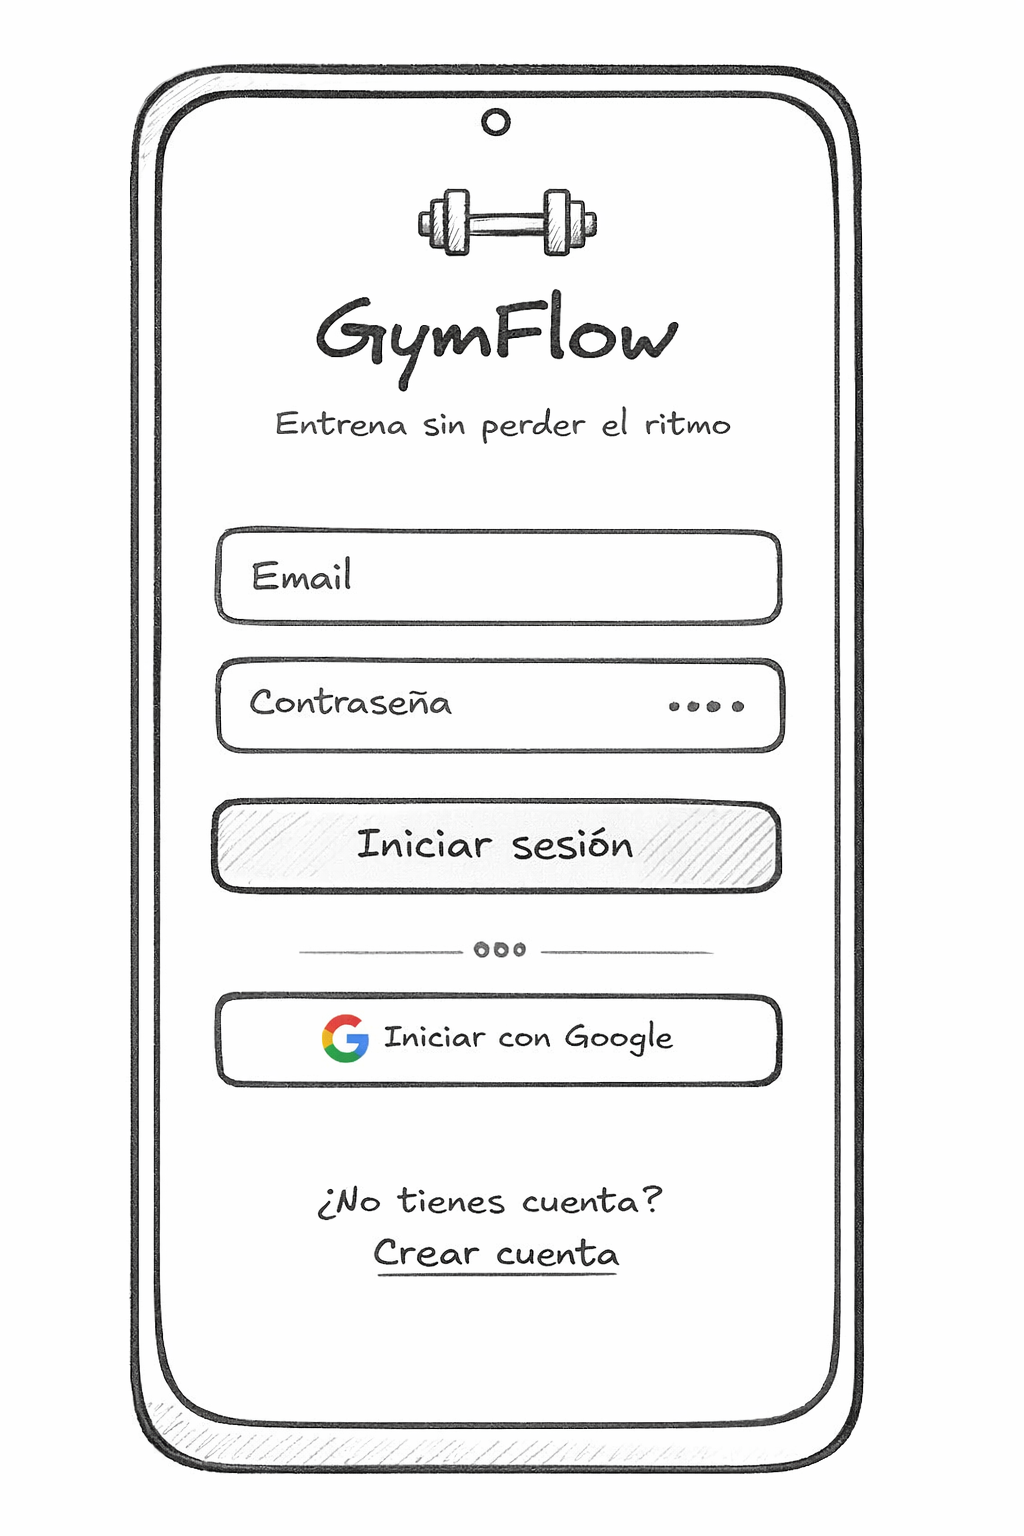
\includegraphics[width=0.35\textwidth]{login.png}
    \caption{Layout de referencia de la pantalla de inicio de sesión (Login).}
    \label{fig:layout-login}
\end{figure}

\begin{figure}[H]
    \centering
    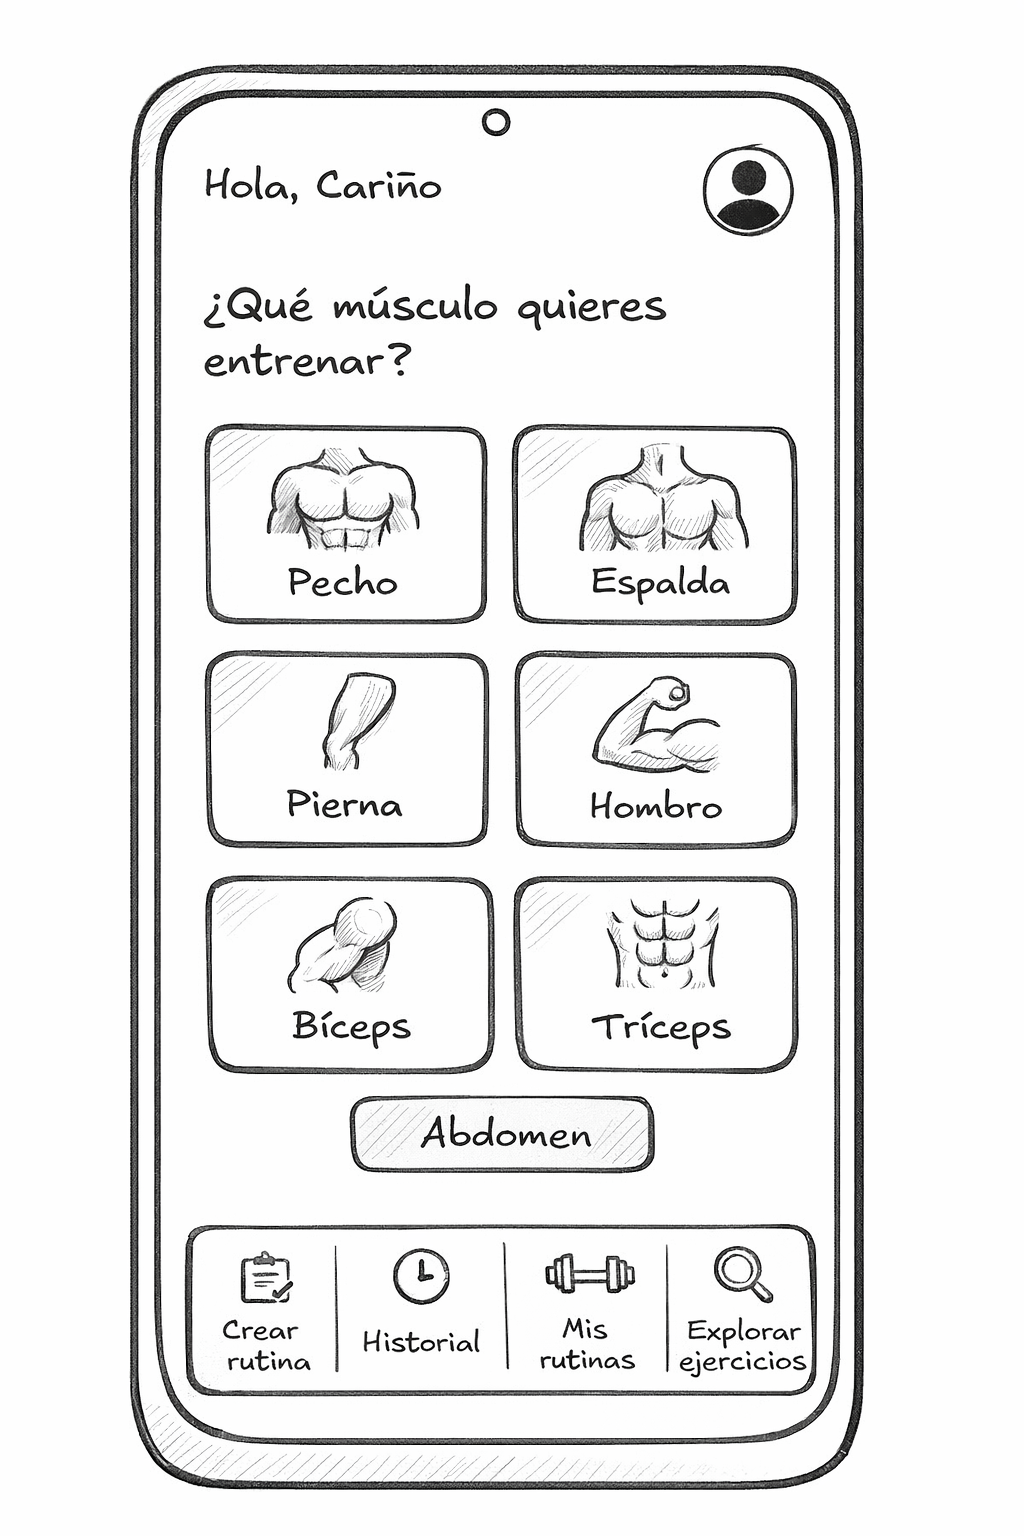
\includegraphics[width=0.35\textwidth]{home.png}
    \caption{Layout de referencia de la pantalla principal de músculos (Home).}
    \label{fig:layout-home}
\end{figure}

\begin{figure}[H]
    \centering
    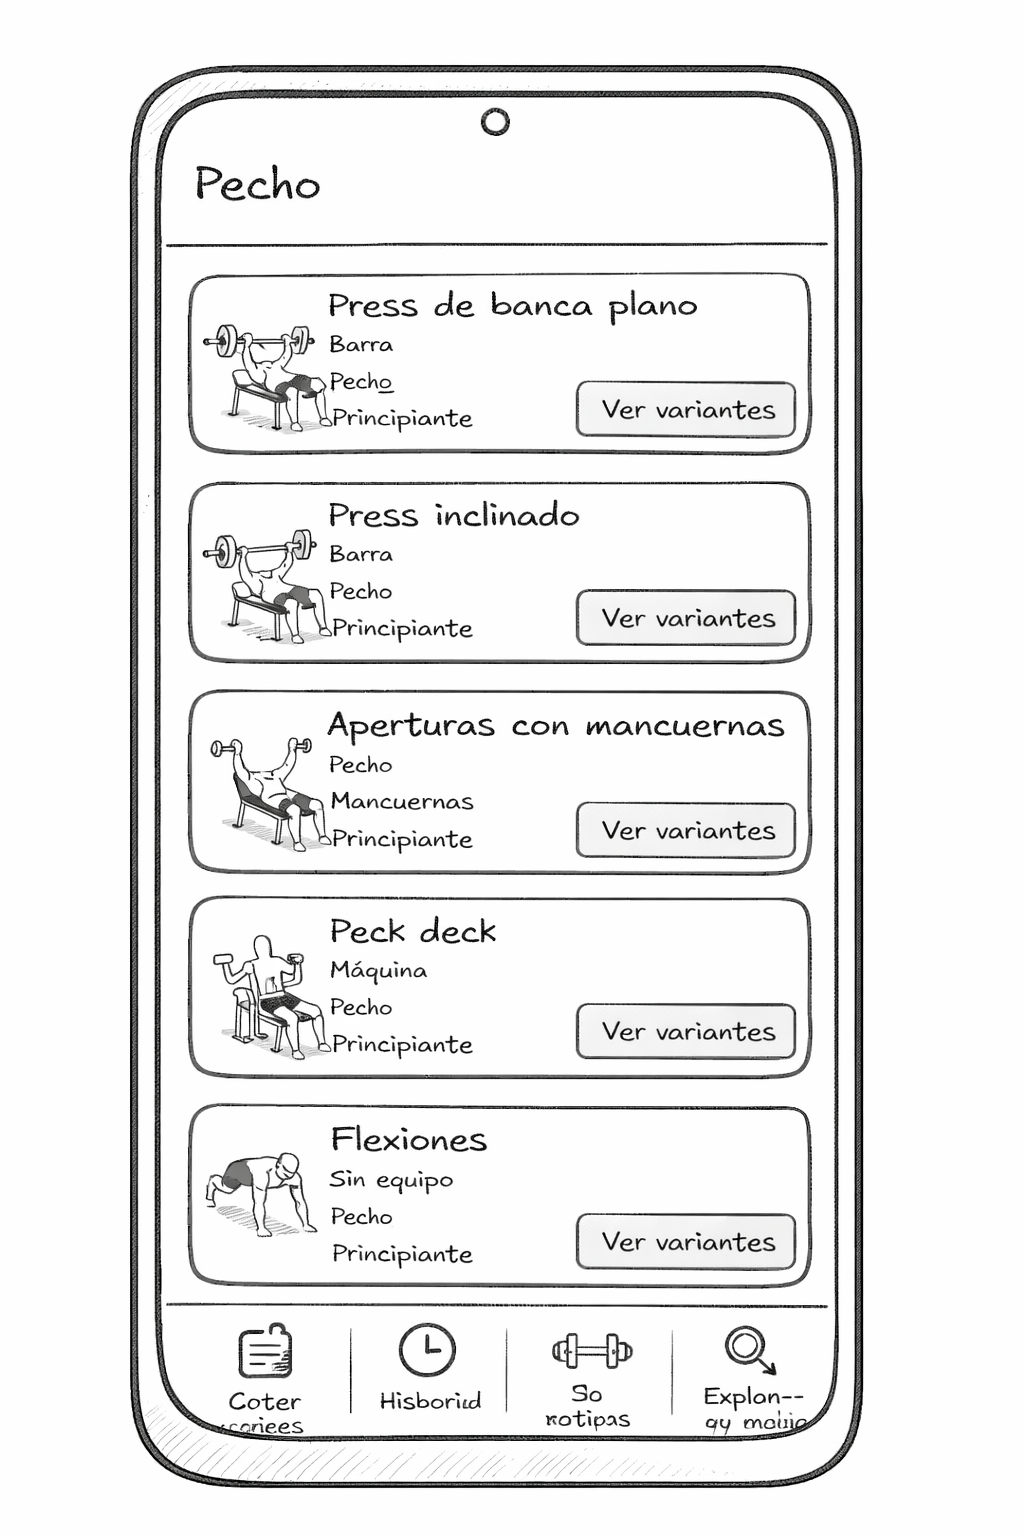
\includegraphics[width=0.35\textwidth]{ejercicios.png}
    \caption{Layout de referencia de la pantalla de ejercicios por músculo.}
    \label{fig:layout-ejercicios}
\end{figure}

\begin{figure}[H]
    \centering
    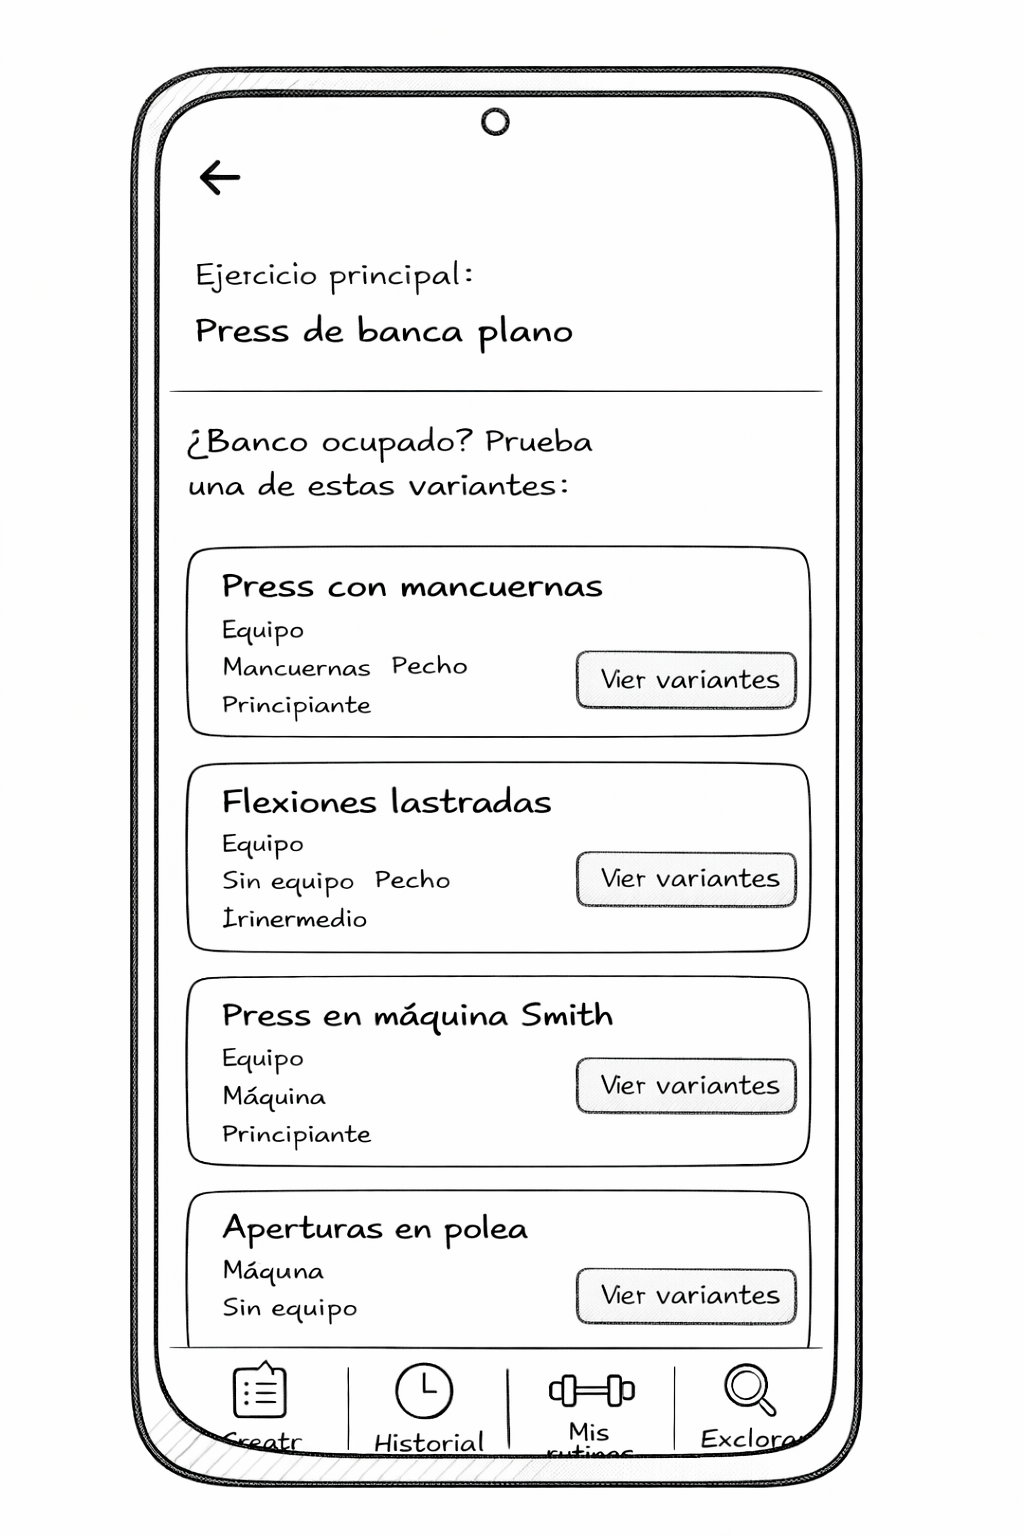
\includegraphics[width=0.35\textwidth]{variantes.png}
    \caption{Layout de referencia de la pantalla de variantes de ejercicio.}
    \label{fig:layout-variantes}
\end{figure}

\begin{figure}[H]
    \centering
    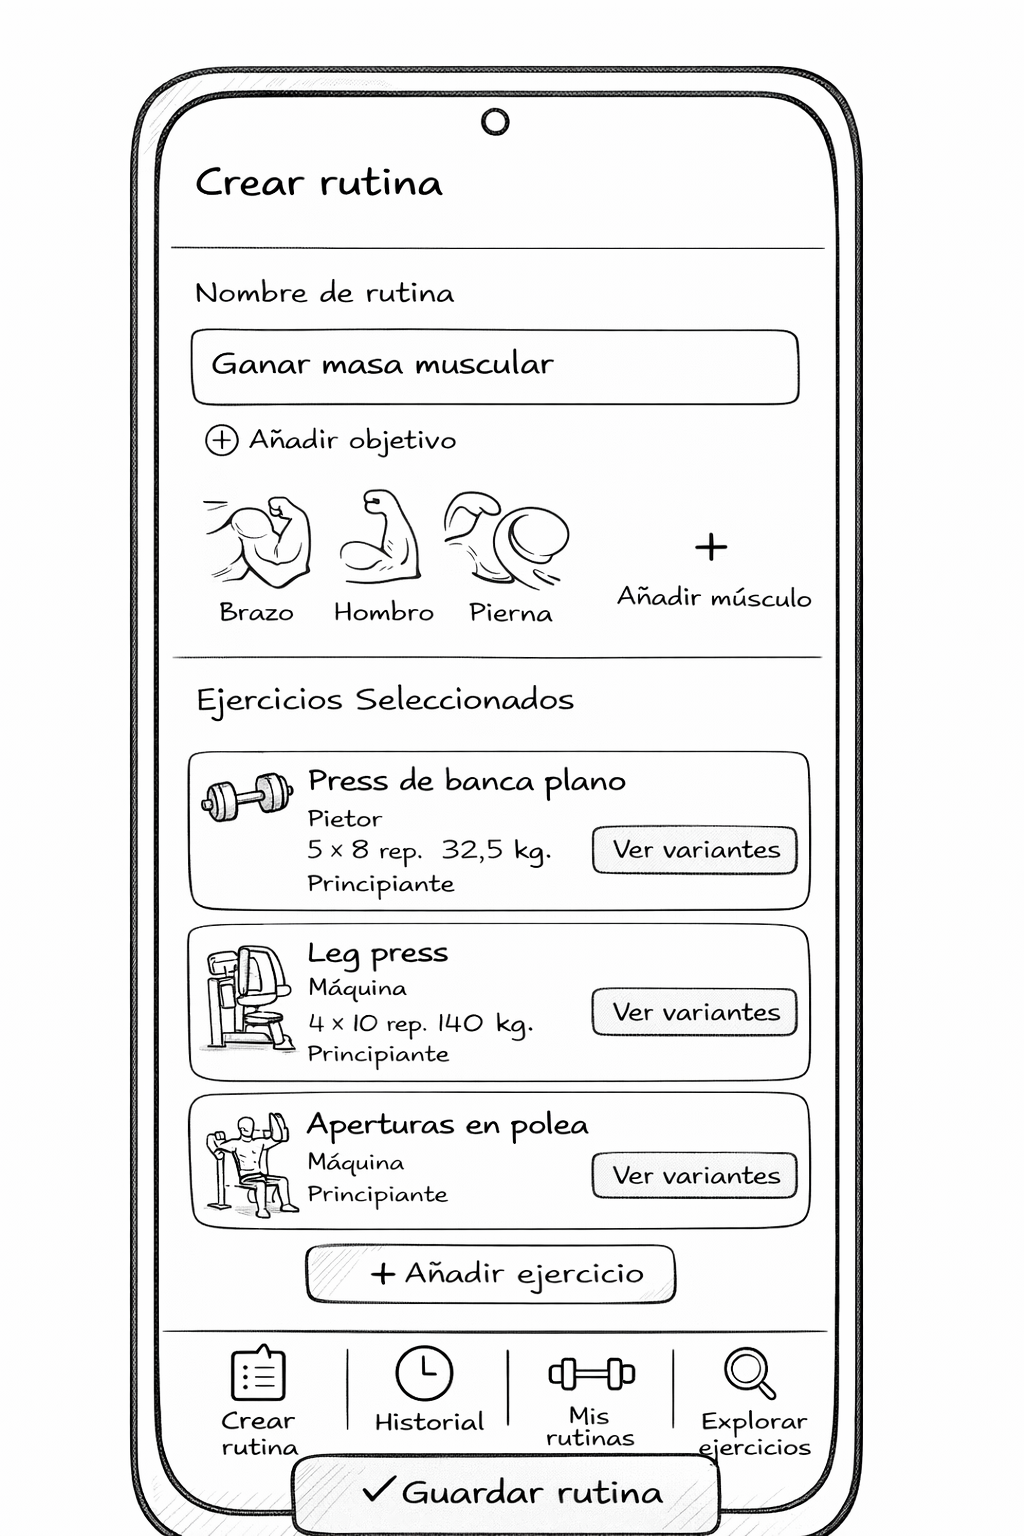
\includegraphics[width=0.35\textwidth]{crear-rutina.png}
    \caption{Layout de referencia de la pantalla de creación de rutina.}
    \label{fig:layout-crear-rutina}
\end{figure}

\begin{figure}[H]
    \centering
    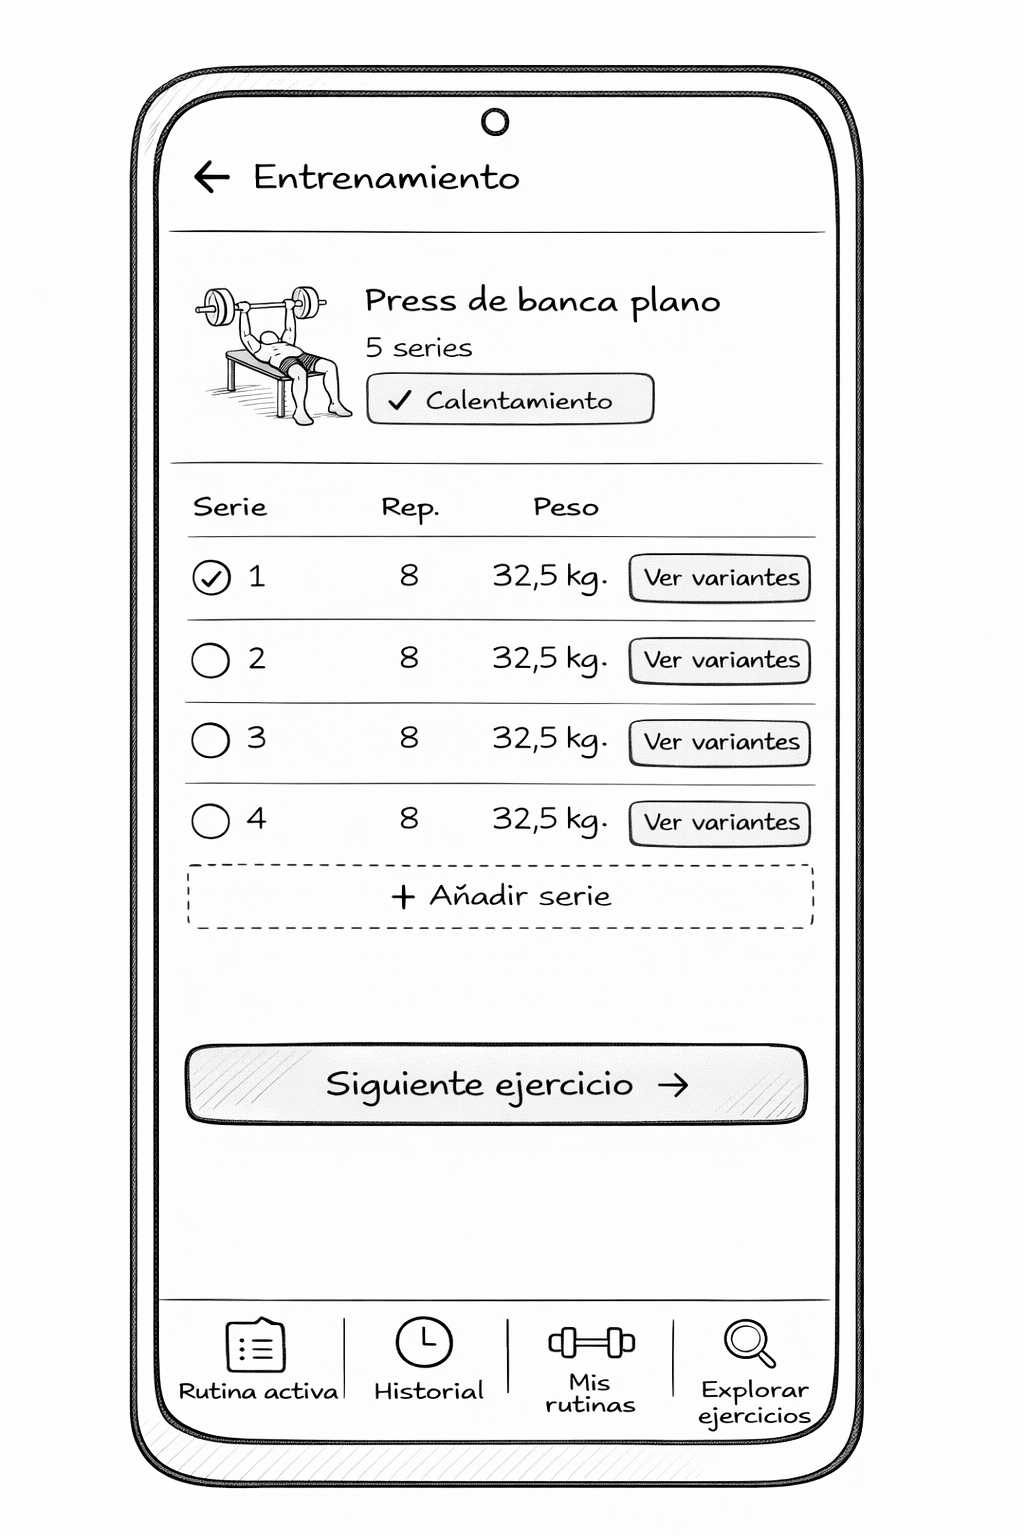
\includegraphics[width=0.35\textwidth]{entrenamiento.png}
    \caption{Layout de referencia de la pantalla de entrenamiento.}
    \label{fig:layout-entrenamiento}
\end{figure}

\begin{figure}[H]
    \centering
    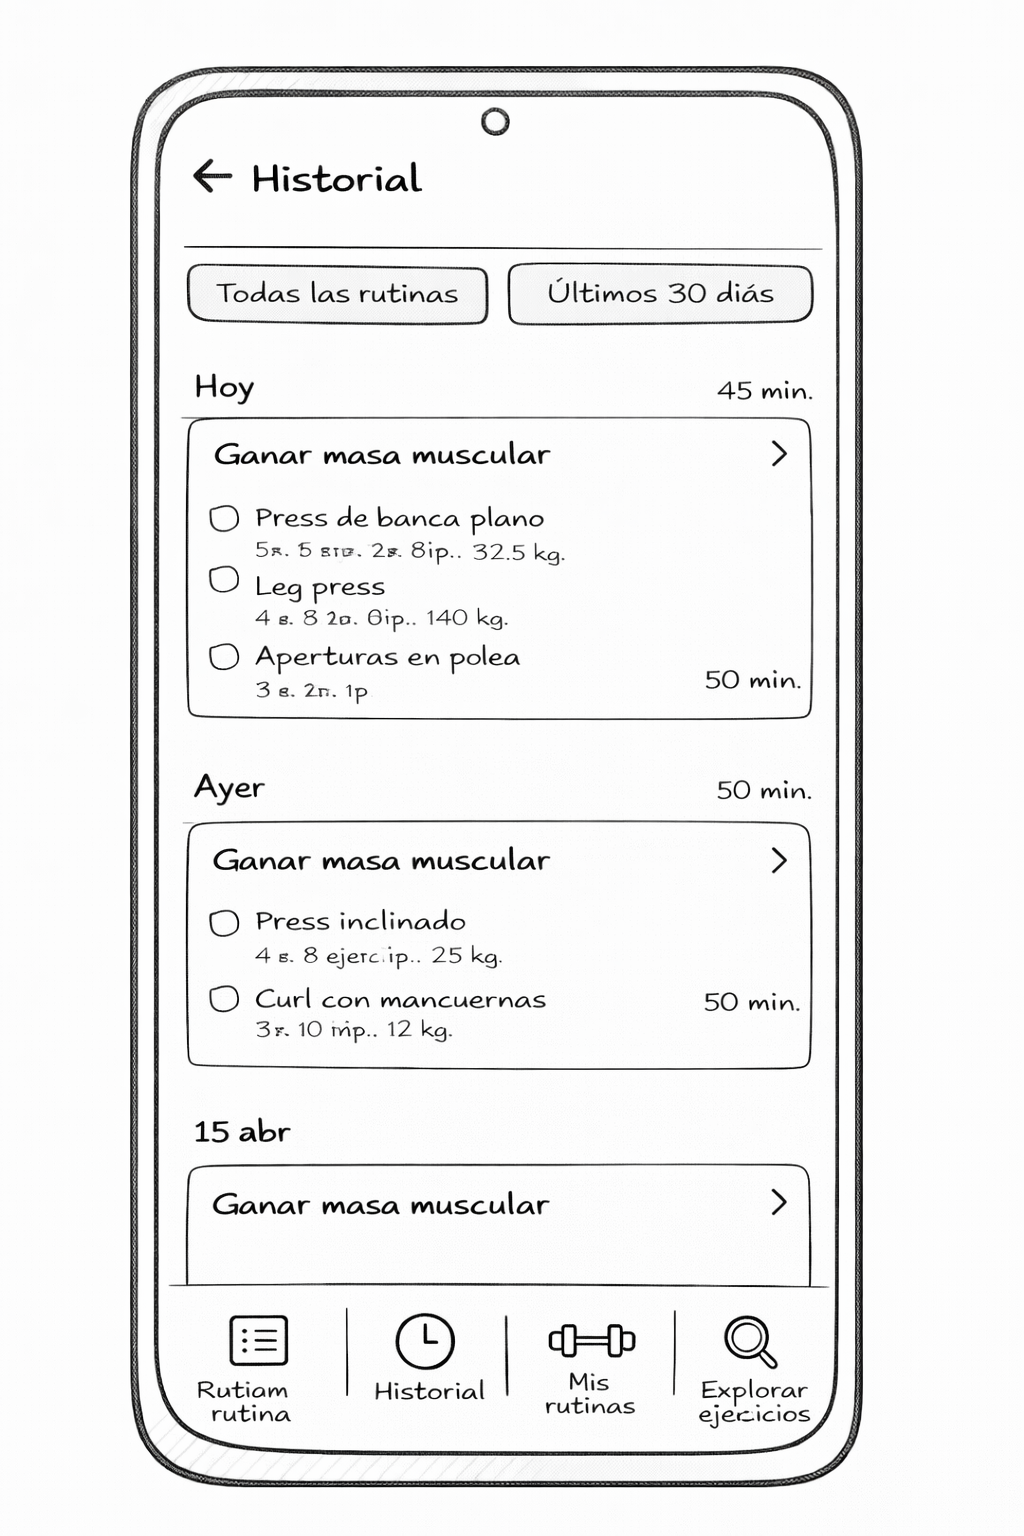
\includegraphics[width=0.35\textwidth]{historial.png}
    \caption{Layout de referencia de la pantalla de historial.}
    \label{fig:layout-historial}
\end{figure}

\subsection{Flujo de navegación del sistema}

El flujo de navegación del sistema describe la manera en que los usuarios interactúan con la aplicación y cómo se conectan las diferentes pantallas. La navegación se implementa con \textit{Expo Router} mediante una pila principal (\textit{Stack}) y una barra de pestañas inferior (\textit{Tabs}). El acceso a las distintas zonas está controlado por dos guardas: una de \textbf{autenticación}, que redirige a los usuarios no autenticados al inicio de sesión, y otra de \textbf{onboarding}, que obliga a completar la configuración inicial del perfil antes de ingresar a la aplicación principal.

\subsubsection{Estructura de navegación}

La aplicación se organiza en cuatro grupos de pantallas, descritos en la Tabla \ref{tab:nav-grupos}.

\begin{table}[H]
\centering
\rowcolors{2}{gymblueSoft}{gymblueSoftAlt}
\arrayrulecolor{gymblue}
\begin{tabularx}{0.98\textwidth}{L{3.6cm} Y}
\toprule
\gymtableheaderrow
\gymth{Grupo / Pantalla} & \gymth{Función dentro de la navegación} \\
\midrule
Acceso (\textit{auth}) & Inicio de sesión y registro, incluido el acceso con Google. \\
Onboarding & Configuración inicial guiada del perfil (objetivo, nivel, días y equipamiento) y elección de la rutina inicial. \\
Pestañas principales & Navegación central de la aplicación: \textit{Hoy}, \textit{Rutinas}, \textit{Historial} y \textit{Músculos}. \\
Pantallas de detalle & Ejercicios por músculo, variantes, creación y edición de rutina, y configuración del perfil. \\
\bottomrule
\end{tabularx}
\caption{Grupos de navegación de la aplicación GymFlow}
\label{tab:nav-grupos}
\end{table}

\subsubsection{Recorrido principal del usuario}

En términos generales, el flujo de interacción sigue la siguiente estructura:

\begin{enumerate}
    \item El usuario inicia sesión con correo y contraseña, o con su cuenta de Google.
    \item Si es la primera vez, completa el \textit{onboarding} y obtiene una rutina inicial activa.
    \item En la pestaña \textit{Hoy} visualiza la sesión del día dentro de su calendario semanal.
    \item Durante la sesión, marca series y ejercicios, registra peso, repeticiones y RPE, reemplaza ejercicios cuando una máquina está ocupada o pospone el día.
    \item Desde la pestaña \textit{Músculos} selecciona un grupo muscular, consulta sus ejercicios y revisa variantes para mantener la continuidad del entrenamiento.
    \item En la pestaña \textit{Rutinas} crea, edita, activa, duplica o archiva sus rutinas.
    \item En la pestaña \textit{Historial} revisa las sesiones realizadas, pospuestas y no realizadas, con el detalle de las series registradas.
\end{enumerate}

Este flujo permite que el usuario continúe su entrenamiento incluso cuando ciertas máquinas o equipos del gimnasio no estén disponibles, ofreciendo alternativas para trabajar el mismo grupo muscular. El siguiente esquema resume la transición entre las zonas principales del sistema.

\begin{figure}[H]
\centering
\footnotesize
\setlength{\fboxsep}{6pt}
\fbox{Inicio} $\rightarrow$ \fbox{Acceso / Registro} $\rightarrow$ \fbox{Onboarding} $\rightarrow$ \fbox{Hoy (sesión)} \\[8pt]
\fbox{Hoy (sesión)} $\leftrightarrow$ \fbox{Rutinas} $\leftrightarrow$ \fbox{Historial} $\leftrightarrow$ \fbox{Músculos} \\[8pt]
\fbox{Músculos} $\rightarrow$ \fbox{Ejercicios por músculo} $\rightarrow$ \fbox{Variantes} \\[8pt]
\fbox{Rutinas} $\rightarrow$ \fbox{Crear / Editar rutina} \qquad \fbox{Perfil} $\rightarrow$ \fbox{Cerrar sesión}
\caption{Esquema del flujo de navegación entre las zonas principales del sistema.}
\label{fig:flujo-navegacion}
\end{figure}

\subsection{Modelo de datos del sistema}

El modelo de datos del sistema organiza la información utilizada por la aplicación. La persistencia se realiza sobre \textit{Cloud Firestore}, donde los datos se dividen en dos ámbitos: un \textbf{catálogo global} compartido por todos los usuarios (músculos, ejercicios, variantes y rutinas prediseñadas) y la \textbf{información personal} de cada usuario, almacenada bajo su identificador (\texttt{users/\{uid\}}). La autenticación y la identidad del usuario son gestionadas por \textit{Firebase Authentication}.

\subsubsection{Entidades principales}

Las entidades del sistema y su contenido se resumen en la Tabla \ref{tab:entidades}.

\begin{table}[H]
\centering
\rowcolors{2}{gymblueSoft}{gymblueSoftAlt}
\arrayrulecolor{gymblue}
\begin{tabularx}{0.98\textwidth}{L{3.4cm} L{3.6cm} Y}
\toprule
\gymtableheaderrow
\gymth{Entidad} & \gymth{Ubicación (colección)} & \gymth{Atributos principales} \\
\midrule
Usuario & Firebase Authentication & Identificador, nombre, correo, foto y proveedor de acceso (correo o Google). \\
Perfil & \texttt{users/\{uid\}/profile} & Objetivo, nivel, días de entrenamiento, equipamiento y estado del onboarding. \\
Músculo & \texttt{muscles} & Nombre, ícono, color e imagen del grupo muscular. \\
Ejercicio & \texttt{exercises} & Músculo asociado, nombre, descripción y equipamiento. \\
Variante & \texttt{variants} & Ejercicio de origen, nombre, descripción y ejercicio sustituto. \\
Rutina prediseñada & \texttt{routine\_templates} & Nombre, descripción, nivel, objetivo, días, equipamiento, división y plan semanal. \\
Rutina & \texttt{users/\{uid\}/routines} & Nombre, ejercicios, estado, plan semanal, días por semana e inicio del ciclo. \\
Día de entrenamiento & \texttt{users/\{uid\}/training\_days} & Fecha, estado del día, ejercicios y series completados. \\
Sesión de entrenamiento & \texttt{users/\{uid\}/workout\_sessions} & Fecha, estado, ejercicios planificados y resultado de la sesión. \\
Registro de ejercicio & \texttt{users/\{uid\}/exercise\_logs} & Fecha, ejercicio y series con peso, repeticiones y RPE. \\
\bottomrule
\end{tabularx}
\caption{Entidades principales del modelo de datos de GymFlow}
\label{tab:entidades}
\end{table}

\subsubsection{Relaciones entre entidades}

Las principales relaciones del modelo se describen en la Tabla \ref{tab:relaciones}.

\begin{table}[H]
\centering
\rowcolors{2}{gymblueSoft}{gymblueSoftAlt}
\arrayrulecolor{gymblue}
\begin{tabularx}{0.98\textwidth}{L{5.2cm} Y}
\toprule
\gymtableheaderrow
\gymth{Relación} & \gymth{Descripción} \\
\midrule
Músculo --- Ejercicio & Un músculo agrupa varios ejercicios; cada ejercicio pertenece a un músculo. \\
Ejercicio --- Variante & Un ejercicio puede tener varias variantes o alternativas para trabajar el mismo músculo. \\
Usuario --- Perfil & Cada usuario posee un único perfil con sus preferencias de entrenamiento. \\
Usuario --- Rutina & Un usuario puede tener varias rutinas, de las cuales como máximo una está activa. \\
Rutina --- Ejercicio & Una rutina referencia un conjunto de ejercicios distribuidos en un plan semanal. \\
Usuario --- Sesión / Registro & Cada usuario genera días y sesiones de entrenamiento, con registros de series por ejercicio y fecha. \\
\bottomrule
\end{tabularx}
\caption{Relaciones entre las entidades del modelo de datos}
\label{tab:relaciones}
\end{table}

Esta organización centraliza la información del catálogo y mantiene aislada la información personal de cada usuario bajo su propio identificador, lo que facilita la seguridad de los datos, la escalabilidad del sistema y la consistencia entre las rutinas, las sesiones y el historial de entrenamiento.

\section{Arquitectura del Sistema}

\subsection{Descripción General de la Arquitectura}

La arquitectura de \textbf{GymFlow} sigue un modelo \textbf{cliente-servidor} basado en servicios en la nube (\textit{Backend as a Service}). Se compone de tres bloques principales: la aplicación móvil (cliente), los servicios de Firebase (servidor) y una capa de almacenamiento local en el dispositivo. El usuario interactúa directamente con la aplicación móvil desarrollada en React Native con Expo, desde donde puede registrarse, iniciar sesión, consultar ejercicios, visualizar variantes, crear rutinas y registrar sus entrenamientos.

La aplicación móvil se integra con \textit{Firebase Authentication} para la gestión del acceso de usuarios, incluido el inicio de sesión con cuenta de Google. La información del sistema se organiza mediante \textit{Cloud Firestore}, donde se almacenan los datos del catálogo (músculos, ejercicios, variantes y rutinas prediseñadas) y la información personal de cada usuario (perfil, rutinas, días y sesiones de entrenamiento e historial). Adicionalmente, la aplicación mantiene una \textbf{caché local} sobre el almacenamiento del dispositivo (\textit{AsyncStorage}) que habilita el funcionamiento sin conexión y la sincronización posterior con Firestore.

De manera general, el flujo de la arquitectura puede representarse así:

\begin{center}
Aplicación móvil (cliente) $\leftrightarrow$ Caché local (AsyncStorage) \\[4pt]
Aplicación móvil $\rightarrow$ Firebase Authentication $\rightarrow$ Cloud Firestore
\end{center}

\subsection{Tecnologías Utilizadas}

El sistema se construyó con un conjunto de tecnologías orientadas al desarrollo móvil multiplataforma y a los servicios en la nube. La Tabla \ref{tab:tecnologias-arq} resume los componentes principales y la tecnología empleada en cada uno.

\begin{table}[H]
\centering
\rowcolors{2}{gymblueSoft}{gymblueSoftAlt}
\arrayrulecolor{gymblue}
\begin{tabularx}{0.92\textwidth}{L{4.2cm} Y}
\toprule
\gymtableheaderrow
\gymth{Componente} & \gymth{Tecnología utilizada} \\
\midrule
Lenguaje & TypeScript \\
Frontend & React Native con Expo \\
Navegación & Expo Router \\
Servicios backend & Firebase (Backend as a Service) \\
Autenticación & Firebase Authentication y Google Sign-In \\
Base de datos principal & Cloud Firestore \\
Persistencia local / offline & AsyncStorage \\
Comunicación cliente-servidor & SDK de Firebase sobre HTTPS \\
\bottomrule
\end{tabularx}
\caption{Tecnologías utilizadas en el sistema GymFlow}
\label{tab:tecnologias-arq}
\end{table}

\subsection{Diagrama de Arquitectura}

\begin{figure}[H]
    \centering
    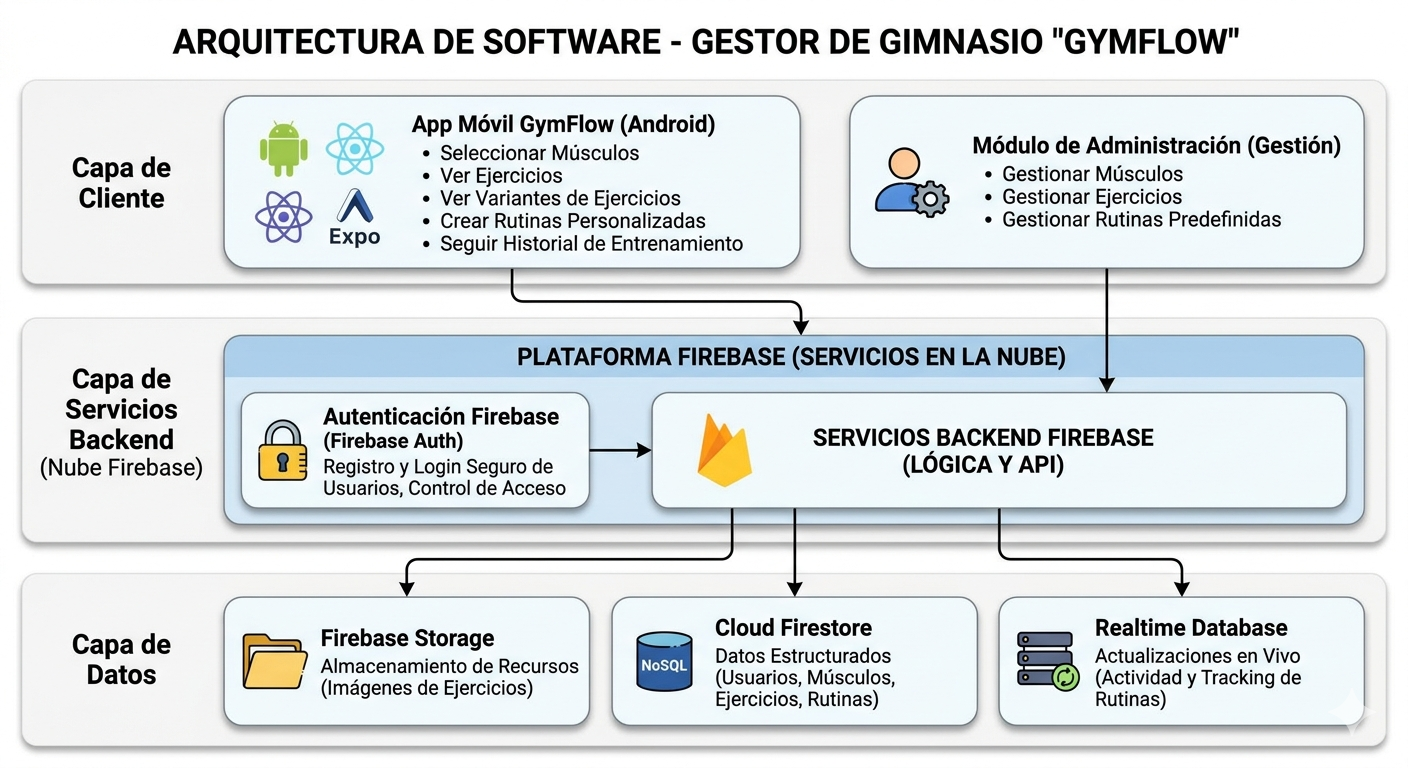
\includegraphics[width=0.85\textwidth]{arquitecture.png}
    \caption{Diagrama de arquitectura del sistema GymFlow}
    \label{fig:arquitectura}
\end{figure}

Esta arquitectura centraliza la información, facilita la autenticación de usuarios y mantiene una estructura flexible para futuras ampliaciones del sistema.

\section{Metodología Aplicada}

Para el desarrollo del proyecto GymFlow se adopta la metodología ágil \textbf{SCRUM}. Esta metodología permite organizar el trabajo en ciclos cortos, priorizar funcionalidades y evaluar avances parciales de forma constante. En el contexto del proyecto, SCRUM resulta adecuado porque facilita ajustar el alcance del producto conforme se validan la interfaz, la navegación, la lógica de rutinas y la integración con Firebase.

El trabajo del equipo se estructura en un \textbf{sprint 0 de planificación} y \textbf{cuatro sprints de desarrollo funcional}. A partir del \textbf{14 de abril de 2026} cada sprint funcional tiene una duración fija de \textbf{14 días calendario}. El \textbf{sprint 0} comenzó el \textbf{martes 7 de abril de 2026}, una semana antes del inicio del sprint 1, con el objetivo de dejar lista la base técnica, organizativa y documental del proyecto. El \textbf{sprint 4} consolida las funcionalidades avanzadas efectivamente implementadas en el sistema (acceso con Google, configuración personalizada del perfil, planificación y ejecución de sesiones de entrenamiento, historial detallado y funcionamiento sin conexión).

\subsection{Ciclo de vida del proyecto}

El desarrollo del sistema se organiza en un ciclo de vida iterativo compuesto por las siguientes fases:

\begin{itemize}
\item \textbf{Planificación:} definición del problema, alcance, objetivos, backlog inicial y organización del equipo.
\item \textbf{Análisis:} identificación de requerimientos funcionales y no funcionales, así como del contexto de uso de la aplicación.
\item \textbf{Diseño:} elaboración de la arquitectura, diagramas, mockups y estructura conceptual de datos.
\item \textbf{Implementación:} desarrollo de la aplicación móvil con React Native, Expo y servicios de Firebase.
\item \textbf{Pruebas:} validación de funcionalidades, revisión de errores y evaluación básica de la experiencia de usuario.
\item \textbf{Despliegue:} preparación de la aplicación para demostración, entrega académica y futuras publicaciones.
\end{itemize}

\subsection{Aplicación de SCRUM en el proyecto}

La aplicación de SCRUM en GymFlow se orienta a mantener un ritmo de trabajo incremental, con revisión continua del backlog y entregables verificables al cierre de cada sprint. Para ello, el proyecto adopta los siguientes elementos metodológicos:

\begin{itemize}
\item \textbf{Product Backlog:} lista priorizada de historias de usuario, tareas técnicas y mejoras del sistema.
\item \textbf{Sprint Backlog:} conjunto de historias y tareas comprometidas para cada sprint de 14 días.
\item \textbf{Incremento:} resultado funcional o verificable entregado al finalizar cada sprint.
\item \textbf{Definition of Done (DoD):} criterio mínimo para considerar una historia como terminada.
\item \textbf{Refinamiento del backlog:} revisión periódica de historias para aclarar alcance, dependencias y criterios de aceptación.
\end{itemize}

\subsection{Eventos SCRUM}

Para sostener la dinámica de trabajo, el equipo considera los siguientes eventos dentro de cada sprint:

\begin{table}[H]
\centering
\rowcolors{2}{gymblueSoft}{gymblueSoftAlt}
\arrayrulecolor{gymblue}
\begin{tabularx}{0.98\textwidth}{L{3.2cm} L{3.2cm} Y}
\toprule
\gymtableheaderrow
\gymth{Evento} & \gymth{Frecuencia} & \gymth{Propósito} \\
\midrule
Sprint Planning & Inicio de cada sprint & Seleccionar historias prioritarias, dividirlas en tareas y definir el objetivo del sprint. \\
Daily Scrum & Diario & Revisar avances, bloqueos y siguientes acciones del equipo. \\
Backlog Refinement & Al menos una vez por sprint & Aclarar historias de usuario, ajustar prioridades y preparar trabajo futuro. \\
Sprint Review & Fin de cada sprint & Presentar el incremento logrado y validar el resultado frente a los objetivos del sprint. \\
Sprint Retrospective & Fin de cada sprint & Identificar mejoras del proceso de trabajo, coordinación y calidad técnica del equipo. \\
\bottomrule
\end{tabularx}
\caption{Eventos SCRUM aplicados al proyecto GymFlow}
\end{table}

\subsection{Product Backlog}

El \textit{Product Backlog} de GymFlow reúne las funcionalidades priorizadas del sistema y organiza el trabajo funcional que será desarrollado entre los sprints 1, 2 y 3. Este backlog se construye a partir del problema central del proyecto: permitir que el usuario continúe su entrenamiento cuando una máquina o ejercicio no está disponible.

\begin{table}[H]
\centering
\rowcolors{2}{gymblueSoft}{gymblueSoftAlt}
\arrayrulecolor{gymblue}
\begin{tabularx}{0.98\textwidth}{L{2.1cm} L{2cm} L{1.8cm} Y}
\toprule
\gymtableheaderrow
\gymth{Historia} & \gymth{Sprint} & \gymth{Prioridad} & \gymth{Resultado esperado} \\
\midrule
HU-01 & Sprint 1 & Alta & Registro de nuevos usuarios en la aplicación. \\
HU-02 & Sprint 1 & Alta & Inicio de sesión seguro con credenciales del usuario. \\
HU-03 & Sprint 1 & Media & Acceso a una pantalla principal clara y funcional. \\
HU-04 & Sprint 2 & Alta & Consulta de grupos musculares disponibles. \\
HU-05 & Sprint 2 & Alta & Visualización de ejercicios asociados a cada músculo. \\
HU-06 & Sprint 2 & Alta & Consulta de variantes para continuidad del entrenamiento. \\
HU-07 & Sprint 3 & Alta & Creación de rutinas personalizadas. \\
HU-08 & Sprint 3 & Alta & Guardado persistente de rutinas del usuario. \\
HU-09 & Sprint 3 & Media & Gestión y consulta de rutinas guardadas. \\
HU-10 & Sprint 3 & Media & Acceso a rutinas prediseñadas. \\
HU-11 & Sprint 4 & Alta & Inicio de sesión con cuenta de Google. \\
HU-12 & Sprint 4 & Alta & Configuración inicial del perfil mediante onboarding guiado. \\
HU-13 & Sprint 4 & Media & Edición del perfil y preferencias de entrenamiento. \\
HU-14 & Sprint 4 & Media & Cierre de sesión del usuario. \\
HU-15 & Sprint 4 & Alta & Activación de una rutina y arranque del ciclo semanal. \\
HU-16 & Sprint 4 & Media & Edición de rutinas existentes. \\
HU-17 & Sprint 4 & Media & Duplicar, archivar y eliminar rutinas. \\
HU-18 & Sprint 4 & Alta & Planificación automática de la rutina por días de la semana. \\
HU-19 & Sprint 4 & Alta & Calendario semanal con días de sesión y descanso. \\
HU-20 & Sprint 4 & Alta & Ejecución de la sesión marcando series y ejercicios. \\
HU-21 & Sprint 4 & Alta & Registro de series con peso, repeticiones y RPE. \\
HU-22 & Sprint 4 & Alta & Reemplazo de un ejercicio durante la sesión activa. \\
HU-23 & Sprint 4 & Media & Posponer un día de entrenamiento. \\
HU-24 & Sprint 4 & Media & Historial detallado de entrenamientos realizados. \\
HU-25 & Sprint 4 & Baja & Consulta de la técnica del ejercicio mediante video. \\
HU-26 & Sprint 4 & Alta & Funcionamiento sin conexión y sincronización de datos. \\
\bottomrule
\end{tabularx}
\caption{Product Backlog del proyecto GymFlow}
\end{table}

\subsection{Sprint Backlog}

El \textit{Sprint Backlog} se define al inicio de cada sprint y contiene las historias comprometidas por el equipo, junto con las tareas técnicas y de validación necesarias para alcanzar el objetivo del sprint.

\begin{table}[H]
\centering
\rowcolors{2}{gymblueSoft}{gymblueSoftAlt}
\arrayrulecolor{gymblue}
\begin{tabularx}{0.98\textwidth}{L{2cm} L{2.4cm} Y}
\toprule
\gymtableheaderrow
\gymth{Sprint} & \gymth{Historias incluidas} & \gymth{Alcance del sprint} \\
\midrule
Sprint 1 & HU-01, HU-02, HU-03 & Implementar autenticación, acceso al sistema y navegación inicial. \\
Sprint 2 & HU-04, HU-05, HU-06 & Resolver la consulta de músculos, ejercicios y variantes como núcleo funcional de GymFlow. \\
Sprint 3 & HU-07, HU-08, HU-09, HU-10 & Desarrollar la creación, almacenamiento, consulta y reutilización de rutinas. \\
Sprint 4 & HU-11 a HU-26 & Consolidar el acceso con Google, el perfil personalizado, la planificación y ejecución de sesiones de entrenamiento, el historial detallado y el funcionamiento sin conexión. \\
\bottomrule
\end{tabularx}
\caption{Sprint Backlog resumido del proyecto GymFlow}
\end{table}

\subsection{Herramientas de Gestión}

Para la organización del proyecto se utilizan herramientas que permiten planificar el trabajo, coordinar tareas y documentar decisiones del equipo.

\begin{table}[H]
\centering
\rowcolors{2}{gymblueSoft}{gymblueSoftAlt}
\arrayrulecolor{gymblue}
\begin{tabularx}{0.95\textwidth}{L{3.5cm} Y}
\toprule
\gymtableheaderrow
\gymth{Herramienta} & \gymth{Uso dentro del proyecto} \\
\midrule
GitHub & Control de versiones del código fuente, respaldo del repositorio y seguimiento de cambios del proyecto. \\
Notion & Organización de tareas, planificación de sprints, priorización del backlog y seguimiento del avance. \\
Excalidraw & Elaboración de diagramas, esquemas de arquitectura y apoyo visual para el diseño del sistema. \\
WhatsApp y Discord & Comunicación y coordinación entre los integrantes del equipo durante el desarrollo. \\
\bottomrule
\end{tabularx}
\caption{Herramientas de gestión utilizadas en el proyecto}
\end{table}

\section{Seguimiento y Desarrollo Grupal}

\subsection{Roles y Responsabilidades}

El equipo de desarrollo está conformado por cuatro integrantes que trabajan de manera colaborativa en la construcción del sistema.

\begin{table}[H]
\centering
\rowcolors{2}{gymblueSoft}{gymblueSoftAlt}
\arrayrulecolor{gymblue}
\begin{tabularx}{0.92\textwidth}{Y L{4.2cm}}
\toprule
\gymtableheaderrow
\gymth{Integrante} & \gymth{Rol} \\
\midrule
Mita Zeballos Cristian Juan & Scrum Master \\
Chamaca Jimenez Cristhian & Desarrollador Full Stack \\
Montaño Frías Andres & Desarrollador Full Stack \\
Zeballos Valencia Reynaldo & Desarrollador Full Stack \\
\bottomrule
\end{tabularx}
\caption{Roles del equipo de desarrollo}
\end{table}

En la dinámica de trabajo, el \textbf{Scrum Master} coordina ceremonias, da seguimiento a impedimentos y promueve el cumplimiento del proceso. Los \textbf{desarrolladores Full Stack} participan en análisis, diseño, implementación, pruebas y documentación, compartiendo responsabilidad sobre el incremento entregado en cada sprint.

\subsection{Control de Versiones}

El control de versiones del proyecto se realiza mediante \textbf{Git} y \textbf{GitHub}. Este mecanismo permite registrar cambios del código fuente, mantener historial del proyecto, coordinar trabajo colaborativo y evitar conflictos al integrar avances de distintos integrantes.

\subsection{Reporte de Avances}

El seguimiento del avance se realiza por sprint y por semana mediante el backlog del proyecto, la documentación del informe y el tablero de trabajo del equipo. Cada incremento se revisa con base en los objetivos del sprint, las historias comprometidas y la evidencia de avance generada durante el desarrollo.

\subsection{Comunicación}

La comunicación y coordinación del equipo se apoyan en \textbf{WhatsApp}, \textbf{Discord} y reuniones de seguimiento. Estas herramientas permiten resolver bloqueos, coordinar actividades, revisar avances y mantener actualizado el estado del trabajo grupal.

\subsection{Criterios de trabajo del sprint}

Para mantener consistencia metodológica, cada sprint se gestiona con los siguientes criterios:

\begin{itemize}
\item Toda historia de usuario debe incluir descripción clara, valor para el usuario y criterios de aceptación verificables.
\item Las historias priorizadas deben poder completarse dentro del sprint asignado.
\item Cada incremento debe quedar integrado en el repositorio y validado funcionalmente.
\item Las decisiones de diseño y cambios relevantes deben quedar documentados en el informe o en las herramientas de gestión del proyecto.
\item Los bloqueos detectados durante el sprint deben registrarse y tratarse en las reuniones de seguimiento.
\end{itemize}

\subsection{Definición de terminado}

Una historia de usuario se considera terminada cuando cumple simultáneamente con las siguientes condiciones:

\begin{itemize}
\item La funcionalidad fue implementada o documentada de acuerdo con el alcance definido.
\item Los criterios de aceptación fueron revisados y validados por el equipo.
\item El código o entregable correspondiente quedó integrado en la base del proyecto sin errores críticos conocidos.
\item La interfaz o flujo asociado mantiene coherencia con el diseño general de GymFlow.
\item La evidencia del avance quedó reflejada en el backlog, el repositorio o el informe del proyecto.
\end{itemize}

\subsection{Planificación del Trabajo}

La planificación del proyecto se divide en un sprint de planificación y tres sprints de construcción funcional. Cada sprint tiene un objetivo principal, un rango de fechas definido y un conjunto de entregables alineados con los requerimientos del sistema.

\begin{table}[H]
\centering
\rowcolors{2}{gymblueSoft}{gymblueSoftAlt}
\arrayrulecolor{gymblue}
\begin{tabularx}{0.98\textwidth}{L{2.1cm} L{3.3cm} Y}
\toprule
\gymtableheaderrow
\gymth{Sprint} & \gymth{Fechas} & \gymth{Objetivo principal} \\
\midrule
Sprint 0 & 7 de abril de 2026 al 13 de abril de 2026 & Planificar el proyecto: definir backlog inicial, consolidar arquitectura, organizar mockups, configurar el repositorio y dejar lista la base técnica para el desarrollo. \\
Sprint 1 & 14 de abril de 2026 al 27 de abril de 2026 & Implementar el acceso de usuarios y dejar operativa la estructura base de navegación de la aplicación. \\
Sprint 2 & 28 de abril de 2026 al 11 de mayo de 2026 & Desarrollar la consulta de grupos musculares, ejercicios y variantes para resolver el problema principal del proyecto. \\
Sprint 3 & 12 de mayo de 2026 al 25 de mayo de 2026 & Construir la gestión de rutinas personalizadas y la disponibilidad de rutinas prediseñadas para el usuario. \\
Sprint 4 & 26 de mayo de 2026 al 8 de junio de 2026 & Incorporar el acceso con Google, el perfil personalizado mediante onboarding, la planificación y ejecución de sesiones de entrenamiento, el historial detallado y el funcionamiento sin conexión. \\
\bottomrule
\end{tabularx}
\caption{Planificación de sprints del proyecto GymFlow}
\end{table}

\subsection{Historias de usuario por sprint}

Las historias de usuario del proyecto se numeran de forma continua para mantener trazabilidad única dentro del \textit{product backlog}. El sprint 0 no contempla historias funcionales, ya que corresponde exclusivamente a planificación. La distribución de las historias de usuario por sprint es la siguiente:

\begin{table}[H]
\centering
\rowcolors{2}{gymblueSoft}{gymblueSoftAlt}
\arrayrulecolor{gymblue}
\begin{tabularx}{0.98\textwidth}{L{2.1cm} L{2.4cm} Y}
\toprule
\gymtableheaderrow
\gymth{Sprint} & \gymth{Historias} & \gymth{Enfoque del sprint} \\
\midrule
Sprint 0 & No aplica & Planificación general, organización técnica, documental y metodológica del proyecto. \\
Sprint 1 & HU-01 a HU-03 & Registro, inicio de sesión y acceso a la pantalla principal del sistema. \\
Sprint 2 & HU-04 a HU-06 & Consulta de músculos, ejercicios y variantes para mantener la continuidad del entrenamiento. \\
Sprint 3 & HU-07 a HU-10 & Creación, almacenamiento, consulta y reutilización de rutinas personalizadas o prediseñadas. \\
Sprint 4 & HU-11 a HU-26 & Acceso con Google, perfil personalizado, planificación y ejecución de sesiones, historial detallado y funcionamiento sin conexión. \\
\bottomrule
\end{tabularx}
\caption{Distribución continua de historias de usuario por sprint}
\end{table}

Esta organización permite que el proyecto avance de forma incremental, partiendo de una base técnica clara en el sprint 0 y cerrando el cronograma previsto el \textbf{8 de junio de 2026} con una versión funcional que abarca la autenticación (incluido el acceso con Google), la consulta de músculos, ejercicios y variantes, la gestión completa de rutinas y la planificación, ejecución y registro de las sesiones de entrenamiento, todo ello con soporte de uso sin conexión.

\subsection{Planificación operativa externa}

La planificación operativa detallada por sprint y por semana se gestiona fuera del informe en un tablero de trabajo tipo Notion. Este tablero complementa la metodología descrita en el documento y permite registrar, para cada integrante, las actividades asignadas y el producto esperado por semana.

\subsection{Especificación de historias de usuario}

Con el fin de formalizar el backlog del proyecto, cada historia de usuario se documenta de manera individual con su identificador continuo, título descriptivo, sprint asignado, prioridad, descripción, tareas y criterios de aceptación. El sprint 0 no incluye historias de usuario, ya que corresponde únicamente a planificación del proyecto. Las historias HU-01 a HU-10 corresponden al alcance inicial del producto, mientras que las historias HU-11 a HU-26 documentan las funcionalidades avanzadas efectivamente construidas en la aplicación; todas ellas se encuentran implementadas en la versión actual del sistema.

\subsubsection{HU-01 Registro de usuarios}
\begin{table}[H]
\centering
\rowcolors{2}{gymblueSoft}{gymblueSoftAlt}
\arrayrulecolor{gymblue}
\begin{tabularx}{0.98\textwidth}{L{4cm} Y}
\toprule
\gymtableheaderrow
\gymth{Campo} & \gymth{Detalle} \\
\midrule
Identificador & HU-01 \\
Título & Registro de usuarios \\
Sprint & Sprint 1 \\
Estado & Implementado \\
Asignado & Chamaca Jimenez Cristhian \\
Esfuerzo & 3 \\
Prioridad & Alta \\
Versión & 1.0.0 \\
Última edición & 14 de abril de 2026 \\
Descripción & Como usuario nuevo, quiero registrarme mediante un formulario de creación de cuenta para comenzar a utilizar GymFlow. \\
Tareas & \storyitems{\item Diseñar la pantalla de registro.\item Definir los campos obligatorios del formulario.\item Integrar el registro con Firebase Authentication.\item Mostrar mensajes de exito o error al usuario.} \\
Criterios de aceptación & \storyitems{\item El sistema debe permitir ingresar los datos minimos para crear una cuenta.\item Debe informarse al usuario si el registro fue exitoso o si ocurrio un error.\item La cuenta registrada debe quedar lista para autenticarse.} \\
\bottomrule
\end{tabularx}
\caption{Especificación de la historia de usuario HU-01}
\end{table}

\begin{figure}[H]
\centering

\includegraphics[width=0.52\textwidth,height=0.68\textheight,keepaspectratio]{registro-usuario.png}
\caption{Mockup asociado a la historia de usuario HU-01.}
\label{fig:hu01-mockup}
\end{figure}

\subsubsection{HU-02 Inicio de sesión}
\begin{table}[H]
\centering
\rowcolors{2}{gymblueSoft}{gymblueSoftAlt}
\arrayrulecolor{gymblue}
\begin{tabularx}{0.98\textwidth}{L{4cm} Y}
\toprule
\gymtableheaderrow
\gymth{Campo} & \gymth{Detalle} \\
\midrule
Identificador & HU-02 \\
Título & Inicio de sesión \\
Sprint & Sprint 1 \\
Estado & Implementado \\
Asignado & Montaño Frías Andres \\
Esfuerzo & 3 \\
Prioridad & Alta \\
Versión & 1.0.0 \\
Última edición & 14 de abril de 2026 \\
Descripción & Como usuario registrado, quiero iniciar sesión de forma segura con mi correo y contraseña para acceder a mi información personal. \\
Tareas & \storyitems{\item Diseñar la pantalla de inicio de sesión.\item Integrar autenticación con correo y contraseña.\item Validar credenciales y manejo de errores.\item Redirigir al usuario autenticado al flujo principal.} \\
Criterios de aceptación & \storyitems{\item El usuario debe poder iniciar sesión con credenciales validas.\item El sistema debe impedir el acceso con credenciales incorrectas.\item Tras autenticarse, el usuario debe acceder al flujo principal.} \\
\bottomrule
\end{tabularx}
\caption{Especificación de la historia de usuario HU-02}
\end{table}

\begin{figure}[H]
\centering
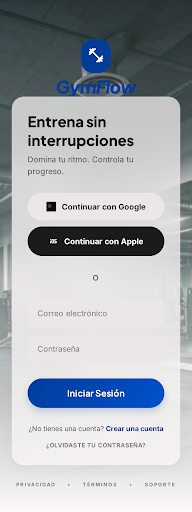
\includegraphics[width=0.52\textwidth,height=0.68\textheight,keepaspectratio]{bienvenida-login.png}
\caption{Mockup asociado a la historia de usuario HU-02.}
\label{fig:hu02-mockup}
\end{figure}

\subsubsection{HU-03 Acceso a pantalla principal}
\begin{table}[H]
\centering
\rowcolors{2}{gymblueSoft}{gymblueSoftAlt}
\arrayrulecolor{gymblue}
\begin{tabularx}{0.98\textwidth}{L{4cm} Y}
\toprule
\gymtableheaderrow
\gymth{Campo} & \gymth{Detalle} \\
\midrule
Identificador & HU-03 \\
Título & Acceso a pantalla principal \\
Sprint & Sprint 1 \\
Estado & Implementado \\
Asignado & Zeballos Valencia Reynaldo \\
Esfuerzo & 2 \\
Prioridad & Media \\
Versión & 1.0.0 \\
Última edición & 14 de abril de 2026 \\
Descripción & Como usuario, quiero ingresar a una pantalla principal clara después del acceso para navegar rapidamente hacia las funciones de entrenamiento. \\
Tareas & \storyitems{\item Diseñar la pantalla principal.\item Organizar accesos a los modulos clave.\item Conectar la navegación inicial con login y registro.\item Validar coherencia con los mockups definidos.} \\
Criterios de aceptación & \storyitems{\item La pantalla posterior al acceso debe mostrar las opciones principales.\item La navegación inicial debe ser clara y consistente con el diseño.\item El usuario debe poder avanzar hacia la consulta de músculos o rutinas sin pasos innecesarios.} \\
\bottomrule
\end{tabularx}
\caption{Especificación de la historia de usuario HU-03}
\end{table}

\begin{figure}[H]
\centering

\includegraphics[width=0.52\textwidth,height=0.68\textheight,keepaspectratio]{dashboard-principal.png}
\caption{Mockup asociado a la historia de usuario HU-03.}
\label{fig:hu03-mockup}
\end{figure}

\subsubsection{HU-04 Consulta de grupos musculares}
\begin{table}[H]
\centering
\rowcolors{2}{gymblueSoft}{gymblueSoftAlt}
\arrayrulecolor{gymblue}
\begin{tabularx}{0.98\textwidth}{L{4cm} Y}
\toprule
\gymtableheaderrow
\gymth{Campo} & \gymth{Detalle} \\
\midrule
Identificador & HU-04 \\
Título & Consulta de grupos musculares \\
Sprint & Sprint 2 \\
Estado & Implementado \\
Asignado & Chamaca Jimenez Cristhian \\
Esfuerzo & 3 \\
Prioridad & Alta \\
Versión & 1.0.0 \\
Última edición & 14 de abril de 2026 \\
Descripción & Como usuario, quiero visualizar los principales grupos musculares para seleccionar con rapidez la zona que deseo entrenar. \\
Tareas & \storyitems{\item Preparar el catalogo base de grupos musculares.\item Diseñar la pantalla de listado de músculos.\item Conectar la consulta con la fuente de datos.\item Validar claridad de la información presentada.} \\
Criterios de aceptación & \storyitems{\item La aplicación debe mostrar una lista de grupos musculares disponibles.\item Cada grupo muscular debe poder seleccionarse desde la interfaz.\item La información mostrada debe ser comprensible para usuarios principiantes e intermedios.} \\
\bottomrule
\end{tabularx}
\caption{Especificación de la historia de usuario HU-04}
\end{table}

\subsubsection{HU-05 Consulta de ejercicios por músculo}
\begin{table}[H]
\centering
\rowcolors{2}{gymblueSoft}{gymblueSoftAlt}
\arrayrulecolor{gymblue}
\begin{tabularx}{0.98\textwidth}{L{4cm} Y}
\toprule
\gymtableheaderrow
\gymth{Campo} & \gymth{Detalle} \\
\midrule
Identificador & HU-05 \\
Título & Consulta de ejercicios por músculo \\
Sprint & Sprint 2 \\
Estado & Implementado \\
Asignado & Montaño Frías Andres \\
Esfuerzo & 3 \\
Prioridad & Alta \\
Versión & 1.0.0 \\
Última edición & 14 de abril de 2026 \\
Descripción & Como usuario, quiero consultar los ejercicios asociados a un músculo especifico para organizar mejor mi sesión de entrenamiento. \\
Tareas & \storyitems{\item Asociar ejercicios a cada grupo muscular.\item Diseñar la vista de ejercicios por músculo.\item Cargar datos segun la selección del usuario.\item Verificar correspondencia entre músculo y ejercicios.} \\
Criterios de aceptación & \storyitems{\item Al seleccionar un músculo, el sistema debe mostrar sus ejercicios asociados.\item La lista de ejercicios debe corresponder al grupo muscular elegido.\item El usuario debe poder continuar desde esa lista hacia la consulta de variantes.} \\
\bottomrule
\end{tabularx}
\caption{Especificación de la historia de usuario HU-05}
\end{table}

\subsubsection{HU-06 Consulta de variantes}
\begin{table}[H]
\centering
\rowcolors{2}{gymblueSoft}{gymblueSoftAlt}
\arrayrulecolor{gymblue}
\begin{tabularx}{0.98\textwidth}{L{4cm} Y}
\toprule
\gymtableheaderrow
\gymth{Campo} & \gymth{Detalle} \\
\midrule
Identificador & HU-06 \\
Título & Consulta de variantes \\
Sprint & Sprint 2 \\
Estado & Implementado \\
Asignado & Chamaca Jimenez Cristhian \\
Esfuerzo & 4 \\
Prioridad & Alta \\
Versión & 1.0.0 \\
Última edición & 14 de abril de 2026 \\
Descripción & Como usuario, quiero ver variantes o ejercicios alternativos cuando una máquina este ocupada para mantener la continuidad de mi rutina. \\
Tareas & \storyitems{\item Definir variantes por ejercicio.\item Diseñar la pantalla de alternativas.\item Conectar el flujo desde ejercicios hacia variantes.\item Validar que las alternativas correspondan al mismo trabajo muscular.} \\
Criterios de aceptación & \storyitems{\item Al seleccionar un ejercicio, el sistema debe mostrar alternativas funcionales para el mismo músculo.\item Las variantes deben presentarse de forma clara y util.\item El flujo debe responder al problema principal de continuidad de la rutina.} \\
\bottomrule
\end{tabularx}
\caption{Especificación de la historia de usuario HU-06}
\end{table}

\subsubsection{HU-07 Creación de rutinas personalizadas}
\begin{table}[H]
\centering
\rowcolors{2}{gymblueSoft}{gymblueSoftAlt}
\arrayrulecolor{gymblue}
\begin{tabularx}{0.98\textwidth}{L{4cm} Y}
\toprule
\gymtableheaderrow
\gymth{Campo} & \gymth{Detalle} \\
\midrule
Identificador & HU-07 \\
Título & Creación de rutinas personalizadas \\
Sprint & Sprint 3 \\
Estado & Implementado \\
Asignado & Chamaca Jimenez Cristhian \\
Esfuerzo & 5 \\
Prioridad & Alta \\
Versión & 1.0.0 \\
Última edición & 14 de abril de 2026 \\
Descripción & Como usuario, quiero crear rutinas de entrenamiento personalizadas seleccionando músculos y ejercicios para adaptar la aplicación a mis objetivos. \\
Tareas & \storyitems{\item Diseñar el flujo de creación de rutina.\item Permitir seleccionar ejercicios.\item Permitir asignar nombre o referencia a la rutina.\item Validar usabilidad del proceso de creación.} \\
Criterios de aceptación & \storyitems{\item El usuario debe poder seleccionar ejercicios para componer una rutina propia.\item La rutina debe permitir identificarse mediante un nombre o referencia.\item El flujo de creación debe ser entendible y consistente con el diseño de la aplicación.} \\
\bottomrule
\end{tabularx}
\caption{Especificación de la historia de usuario HU-07}
\end{table}

\subsubsection{HU-08 Guardado de rutinas}
\begin{table}[H]
\centering
\rowcolors{2}{gymblueSoft}{gymblueSoftAlt}
\arrayrulecolor{gymblue}
\begin{tabularx}{0.98\textwidth}{L{4cm} Y}
\toprule
\gymtableheaderrow
\gymth{Campo} & \gymth{Detalle} \\
\midrule
Identificador & HU-08 \\
Título & Guardado de rutinas \\
Sprint & Sprint 3 \\
Estado & Implementado \\
Asignado & Montaño Frías Andres \\
Esfuerzo & 3 \\
Prioridad & Alta \\
Versión & 1.0.0 \\
Última edición & 14 de abril de 2026 \\
Descripción & Como usuario, quiero guardar mis rutinas para utilizarlas posteriormente sin tener que configurarlas nuevamente. \\
Tareas & \storyitems{\item Definir la estructura de almacenamiento de rutinas.\item Persistir rutinas por usuario.\item Confirmar guardado exitoso.\item Verificar recuperacion posterior de la información.} \\
Criterios de aceptación & \storyitems{\item El sistema debe almacenar la rutina creada por el usuario.\item La rutina guardada debe permanecer asociada a la cuenta correspondiente.\item El usuario debe poder reutilizar esa rutina en un acceso posterior.} \\
\bottomrule
\end{tabularx}
\caption{Especificación de la historia de usuario HU-08}
\end{table}

\subsubsection{HU-09 Gestión de rutinas guardadas}
\begin{table}[H]
\centering
\rowcolors{2}{gymblueSoft}{gymblueSoftAlt}
\arrayrulecolor{gymblue}
\begin{tabularx}{0.98\textwidth}{L{4cm} Y}
\toprule
\gymtableheaderrow
\gymth{Campo} & \gymth{Detalle} \\
\midrule
Identificador & HU-09 \\
Título & Gestión de rutinas guardadas \\
Sprint & Sprint 3 \\
Estado & Implementado \\
Asignado & Zeballos Valencia Reynaldo \\
Esfuerzo & 3 \\
Prioridad & Media \\
Versión & 1.0.0 \\
Última edición & 14 de abril de 2026 \\
Descripción & Como usuario, quiero consultar y gestionar mis rutinas guardadas para editar, reutilizar o reorganizar mi planificación de entrenamiento. \\
Tareas & \storyitems{\item Diseñar la pantalla de listado de rutinas.\item Mostrar detalle de cada rutina guardada.\item Permitir revision y reorganizacion de la información.\item Mantener trazabilidad de cambios por usuario.} \\
Criterios de aceptación & \storyitems{\item El sistema debe mostrar la lista de rutinas guardadas por el usuario.\item El usuario debe poder consultar los detalles de cada rutina almacenada.\item La gestión de rutinas debe permitir al menos revisar y reorganizar la información guardada.} \\
\bottomrule
\end{tabularx}
\caption{Especificación de la historia de usuario HU-09}
\end{table}

\subsubsection{HU-10 Rutinas prediseñadas}
\begin{table}[H]
\centering
\rowcolors{2}{gymblueSoft}{gymblueSoftAlt}
\arrayrulecolor{gymblue}
\begin{tabularx}{0.98\textwidth}{L{4cm} Y}
\toprule
\gymtableheaderrow
\gymth{Campo} & \gymth{Detalle} \\
\midrule
Identificador & HU-10 \\
Título & Rutinas prediseñadas \\
Sprint & Sprint 3 \\
Estado & Implementado \\
Asignado & Montaño Frías Andres \\
Esfuerzo & 2 \\
Prioridad & Media \\
Versión & 1.0.0 \\
Última edición & 14 de abril de 2026 \\
Descripción & Como usuario, quiero acceder a rutinas prediseñadas para disponer de una guía rápida cuando no tenga una rutina propia definida. \\
Tareas & \storyitems{\item Definir un conjunto base de rutinas prediseñadas.\item Diseñar la vista de consulta de rutinas sugeridas.\item Relacionar las rutinas con músculos y ejercicios definidos.\item Permitir su selección como apoyo para el entrenamiento.} \\
Criterios de aceptación & \storyitems{\item La aplicación debe ofrecer un conjunto basico de rutinas prediseñadas.\item El usuario debe poder visualizarlas y seleccionarlas como apoyo.\item Las rutinas prediseñadas deben ser coherentes con los grupos musculares y ejercicios definidos en el sistema.} \\
\bottomrule
\end{tabularx}
\caption{Especificación de la historia de usuario HU-10}
\end{table}

\subsubsection{HU-11 Inicio de sesión con Google}
\begin{table}[H]
\centering
\rowcolors{2}{gymblueSoft}{gymblueSoftAlt}
\arrayrulecolor{gymblue}
\begin{tabularx}{0.98\textwidth}{L{4cm} Y}
\toprule
\gymtableheaderrow
\gymth{Campo} & \gymth{Detalle} \\
\midrule
Identificador & HU-11 \\
Título & Inicio de sesión con Google \\
Sprint & Sprint 4 \\
Estado & Implementado \\
Asignado & Montaño Frías Andres \\
Esfuerzo & 3 \\
Prioridad & Alta \\
Versión & 1.0.0 \\
Última edición & 26 de mayo de 2026 \\
Descripción & Como usuario, quiero iniciar sesión con mi cuenta de Google para acceder a la aplicación de forma rápida sin recordar otra contraseña. \\
Tareas & \storyitems{\item Integrar el inicio de sesión de Google con Firebase Authentication.\item Configurar el cliente de Google Sign-In con el identificador web.\item Convertir el token de Google en una credencial valida para Firebase.\item Manejar la cancelación del usuario y los errores de acceso.} \\
Criterios de aceptación & \storyitems{\item El usuario debe poder autenticarse seleccionando una cuenta de Google.\item La sesión con Google debe quedar asociada al mismo flujo de usuario que el acceso con correo.\item Si el usuario cancela el acceso, el sistema no debe mostrar un error inesperado.} \\
\bottomrule
\end{tabularx}
\caption{Especificación de la historia de usuario HU-11}
\end{table}

\subsubsection{HU-12 Configuracion inicial del perfil (onboarding)}
\begin{table}[H]
\centering
\rowcolors{2}{gymblueSoft}{gymblueSoftAlt}
\arrayrulecolor{gymblue}
\begin{tabularx}{0.98\textwidth}{L{4cm} Y}
\toprule
\gymtableheaderrow
\gymth{Campo} & \gymth{Detalle} \\
\midrule
Identificador & HU-12 \\
Título & Configuracion inicial del perfil (onboarding) \\
Sprint & Sprint 4 \\
Estado & Implementado \\
Asignado & Chamaca Jimenez Cristhian \\
Esfuerzo & 5 \\
Prioridad & Alta \\
Versión & 1.0.0 \\
Última edición & 26 de mayo de 2026 \\
Descripción & Como usuario nuevo, quiero responder unas pocas preguntas sobre mi objetivo, nivel, días disponibles y equipamiento para recibir rutinas que se ajusten a mi situacion. \\
Tareas & \storyitems{\item Diseñar el flujo guiado de cinco pasos (objetivo, nivel, días, equipamiento y eleccion de rutina).\item Guardar el perfil del usuario con sus preferencias.\item Sugerir rutinas prediseñadas acordes al perfil indicado.\item Activar la rutina elegida y marcar el onboarding como completado.} \\
Criterios de aceptación & \storyitems{\item El usuario debe poder avanzar y retroceder entre los pasos del onboarding.\item Las rutinas sugeridas deben corresponder al objetivo, nivel, días y equipamiento elegidos.\item Al finalizar, el perfil debe quedar guardado y la rutina seleccionada debe quedar activa.} \\
\bottomrule
\end{tabularx}
\caption{Especificación de la historia de usuario HU-12}
\end{table}

\subsubsection{HU-13 Edicion del perfil y preferencias}
\begin{table}[H]
\centering
\rowcolors{2}{gymblueSoft}{gymblueSoftAlt}
\arrayrulecolor{gymblue}
\begin{tabularx}{0.98\textwidth}{L{4cm} Y}
\toprule
\gymtableheaderrow
\gymth{Campo} & \gymth{Detalle} \\
\midrule
Identificador & HU-13 \\
Título & Edicion del perfil y preferencias \\
Sprint & Sprint 4 \\
Estado & Implementado \\
Asignado & Zeballos Valencia Reynaldo \\
Esfuerzo & 3 \\
Prioridad & Media \\
Versión & 1.0.0 \\
Última edición & 26 de mayo de 2026 \\
Descripción & Como usuario, quiero modificar mi objetivo, nivel, días disponibles y equipamiento desde la pantalla de perfil para mantener la aplicación alineada con mis necesidades actuales. \\
Tareas & \storyitems{\item Mostrar los datos del usuario (nombre, correo y foto) en la pantalla de perfil.\item Permitir editar objetivo, nivel, días de entrenamiento y equipamiento.\item Guardar los cambios de forma automatica con retroalimentación al usuario.\item Reflejar las preferencias actualizadas en la planificación del entrenamiento.} \\
Criterios de aceptación & \storyitems{\item El usuario debe poder cambiar cualquiera de sus preferencias y verlas reflejadas.\item Los cambios deben guardarse sin requerir un boton de confirmacion explicito.\item Si el guardado falla, el sistema debe informarlo al usuario.} \\
\bottomrule
\end{tabularx}
\caption{Especificación de la historia de usuario HU-13}
\end{table}

\subsubsection{HU-14 Cierre de sesión}
\begin{table}[H]
\centering
\rowcolors{2}{gymblueSoft}{gymblueSoftAlt}
\arrayrulecolor{gymblue}
\begin{tabularx}{0.98\textwidth}{L{4cm} Y}
\toprule
\gymtableheaderrow
\gymth{Campo} & \gymth{Detalle} \\
\midrule
Identificador & HU-14 \\
Título & Cierre de sesión \\
Sprint & Sprint 4 \\
Estado & Implementado \\
Asignado & Zeballos Valencia Reynaldo \\
Esfuerzo & 1 \\
Prioridad & Media \\
Versión & 1.0.0 \\
Última edición & 26 de mayo de 2026 \\
Descripción & Como usuario, quiero cerrar mi sesión desde la pantalla de perfil para proteger mi cuenta cuando dejo de usar la aplicación. \\
Tareas & \storyitems{\item Agregar la accion de cierre de sesión en la pantalla de perfil.\item Cerrar la sesión de Firebase y de Google al salir.\item Redirigir al usuario al flujo de acceso tras cerrar sesión.} \\
Criterios de aceptación & \storyitems{\item El usuario debe poder cerrar sesión desde la pantalla de perfil.\item Tras cerrar sesión, no debe poder accederse a la información personal sin volver a autenticarse.\item El cierre de sesión debe cubrir tanto el acceso con correo como el acceso con Google.} \\
\bottomrule
\end{tabularx}
\caption{Especificación de la historia de usuario HU-14}
\end{table}

\subsubsection{HU-15 Activacion de rutina y ciclo semanal}
\begin{table}[H]
\centering
\rowcolors{2}{gymblueSoft}{gymblueSoftAlt}
\arrayrulecolor{gymblue}
\begin{tabularx}{0.98\textwidth}{L{4cm} Y}
\toprule
\gymtableheaderrow
\gymth{Campo} & \gymth{Detalle} \\
\midrule
Identificador & HU-15 \\
Título & Activacion de rutina y ciclo semanal \\
Sprint & Sprint 4 \\
Estado & Implementado \\
Asignado & Chamaca Jimenez Cristhian \\
Esfuerzo & 4 \\
Prioridad & Alta \\
Versión & 1.0.0 \\
Última edición & 26 de mayo de 2026 \\
Descripción & Como usuario, quiero activar una rutina para que se convierta en mi plan vigente y se inicie un nuevo ciclo semanal de entrenamiento. \\
Tareas & \storyitems{\item Permitir marcar una rutina como activa.\item Asegurar que solo exista una rutina activa a la vez.\item Registrar la fecha de inicio del ciclo de la rutina activa.\item Reiniciar el calendario de la semana al activar una nueva rutina.} \\
Criterios de aceptación & \storyitems{\item Al activar una rutina, cualquier otra rutina activa debe dejar de estarlo.\item El sistema debe registrar el inicio del ciclo para calcular las sesiones de la semana.\item El calendario de entrenamiento debe reflejar la rutina recien activada.} \\
\bottomrule
\end{tabularx}
\caption{Especificación de la historia de usuario HU-15}
\end{table}

\subsubsection{HU-16 Edicion de rutinas}
\begin{table}[H]
\centering
\rowcolors{2}{gymblueSoft}{gymblueSoftAlt}
\arrayrulecolor{gymblue}
\begin{tabularx}{0.98\textwidth}{L{4cm} Y}
\toprule
\gymtableheaderrow
\gymth{Campo} & \gymth{Detalle} \\
\midrule
Identificador & HU-16 \\
Título & Edicion de rutinas \\
Sprint & Sprint 4 \\
Estado & Implementado \\
Asignado & Montaño Frías Andres \\
Esfuerzo & 3 \\
Prioridad & Media \\
Versión & 1.0.0 \\
Última edición & 26 de mayo de 2026 \\
Descripción & Como usuario, quiero editar una rutina existente para ajustar su nombre, ejercicios y días de entrenamiento sin tener que crearla de nuevo. \\
Tareas & \storyitems{\item Diseñar la pantalla de edición de rutina.\item Permitir modificar nombre, ejercicios y días por semana.\item Recalcular la planificación semanal al guardar los cambios.\item Reiniciar el ciclo de la semana si la rutina editada estaba activa.} \\
Criterios de aceptación & \storyitems{\item El usuario debe poder modificar los datos de una rutina guardada.\item Los cambios deben persistir y reflejarse al volver a consultar la rutina.\item Si la rutina editada estaba activa, el calendario debe actualizarse en consecuencia.} \\
\bottomrule
\end{tabularx}
\caption{Especificación de la historia de usuario HU-16}
\end{table}

\subsubsection{HU-17 Duplicar, archivar y eliminar rutinas}
\begin{table}[H]
\centering
\rowcolors{2}{gymblueSoft}{gymblueSoftAlt}
\arrayrulecolor{gymblue}
\begin{tabularx}{0.98\textwidth}{L{4cm} Y}
\toprule
\gymtableheaderrow
\gymth{Campo} & \gymth{Detalle} \\
\midrule
Identificador & HU-17 \\
Título & Duplicar, archivar y eliminar rutinas \\
Sprint & Sprint 4 \\
Estado & Implementado \\
Asignado & Zeballos Valencia Reynaldo \\
Esfuerzo & 3 \\
Prioridad & Media \\
Versión & 1.0.0 \\
Última edición & 26 de mayo de 2026 \\
Descripción & Como usuario, quiero duplicar, archivar o eliminar mis rutinas para organizar mi coleccion de planes segun los uso. \\
Tareas & \storyitems{\item Permitir duplicar una rutina como copia editable.\item Permitir archivar rutinas que ya no se usan de forma activa.\item Permitir eliminar definitivamente una rutina.\item Mantener la consistencia del estado de la rutina activa al realizar estas acciones.} \\
Criterios de aceptación & \storyitems{\item Al duplicar una rutina se debe crear una copia independiente del original.\item Las rutinas archivadas deben dejar de aparecer como opciones activas.\item La eliminacion debe quitar la rutina del listado del usuario.} \\
\bottomrule
\end{tabularx}
\caption{Especificación de la historia de usuario HU-17}
\end{table}

\subsubsection{HU-18 Planificacion automatica de la rutina semanal}
\begin{table}[H]
\centering
\rowcolors{2}{gymblueSoft}{gymblueSoftAlt}
\arrayrulecolor{gymblue}
\begin{tabularx}{0.98\textwidth}{L{4cm} Y}
\toprule
\gymtableheaderrow
\gymth{Campo} & \gymth{Detalle} \\
\midrule
Identificador & HU-18 \\
Título & Planificacion automatica de la rutina semanal \\
Sprint & Sprint 4 \\
Estado & Implementado \\
Asignado & Chamaca Jimenez Cristhian \\
Esfuerzo & 5 \\
Prioridad & Alta \\
Versión & 1.0.0 \\
Última edición & 26 de mayo de 2026 \\
Descripción & Como usuario, quiero que la aplicación distribuya automaticamente los ejercicios de mi rutina en sesiones segun los días que puedo entrenar para no tener que organizarlas manualmente. \\
Tareas & \storyitems{\item Generar un plan semanal a partir de los ejercicios y los días de entrenamiento.\item Asignar series, repeticiones y enfoque muscular a cada sesión.\item Adaptar el plan a los días de la semana realmente seleccionados por el usuario.\item Mantener coherencia entre la rutina activa y la distribución de sesiones.} \\
Criterios de aceptación & \storyitems{\item La rutina activa debe distribuirse en la cantidad de sesiones correspondiente a los días elegidos.\item Cada sesión debe presentar sus ejercicios con series y repeticiones definidas.\item El plan debe ajustarse cuando el usuario cambia sus días disponibles.} \\
\bottomrule
\end{tabularx}
\caption{Especificación de la historia de usuario HU-18}
\end{table}

\subsubsection{HU-19 Calendario semanal de entrenamiento}
\begin{table}[H]
\centering
\rowcolors{2}{gymblueSoft}{gymblueSoftAlt}
\arrayrulecolor{gymblue}
\begin{tabularx}{0.98\textwidth}{L{4cm} Y}
\toprule
\gymtableheaderrow
\gymth{Campo} & \gymth{Detalle} \\
\midrule
Identificador & HU-19 \\
Título & Calendario semanal de entrenamiento \\
Sprint & Sprint 4 \\
Estado & Implementado \\
Asignado & Zeballos Valencia Reynaldo \\
Esfuerzo & 4 \\
Prioridad & Alta \\
Versión & 1.0.0 \\
Última edición & 26 de mayo de 2026 \\
Descripción & Como usuario, quiero ver mi semana de entrenamiento con los días de sesión y de descanso para saber que me toca entrenar cada dia. \\
Tareas & \storyitems{\item Construir la vista semanal de lunes a domingo.\item Diferenciar días de sesión, de descanso, completados, parciales y no realizados.\item Resaltar el dia actual y la sesión correspondiente.\item Derivar el estado de cada dia a partir del ciclo de la rutina activa.} \\
Criterios de aceptación & \storyitems{\item El calendario debe mostrar claramente que días son de entrenamiento y cuales de descanso.\item El dia actual debe identificarse de forma destacada.\item El estado de cada dia debe reflejar el avance real de la sesión.} \\
\bottomrule
\end{tabularx}
\caption{Especificación de la historia de usuario HU-19}
\end{table}

\subsubsection{HU-20 Ejecucion de la sesión: marcar series y ejercicios}
\begin{table}[H]
\centering
\rowcolors{2}{gymblueSoft}{gymblueSoftAlt}
\arrayrulecolor{gymblue}
\begin{tabularx}{0.98\textwidth}{L{4cm} Y}
\toprule
\gymtableheaderrow
\gymth{Campo} & \gymth{Detalle} \\
\midrule
Identificador & HU-20 \\
Título & Ejecucion de la sesión: marcar series y ejercicios \\
Sprint & Sprint 4 \\
Estado & Implementado \\
Asignado & Chamaca Jimenez Cristhian \\
Esfuerzo & 5 \\
Prioridad & Alta \\
Versión & 1.0.0 \\
Última edición & 26 de mayo de 2026 \\
Descripción & Como usuario, quiero marcar mis series y ejercicios como realizados durante la sesión del dia para llevar el control de mi avance en tiempo real. \\
Tareas & \storyitems{\item Permitir marcar y desmarcar series individuales por ejercicio.\item Permitir marcar un ejercicio completo de una sola accion.\item Calcular el estado del dia (pendiente, parcial o completado) segun las series marcadas.\item Restringir el marcado al dia actual y a días no cerrados.} \\
Criterios de aceptación & \storyitems{\item El usuario debe poder marcar series una a una y ver el progreso del ejercicio.\item Un dia debe quedar completado cuando todos sus ejercicios estan marcados.\item No debe permitirse marcar series en días de descanso, pospuestos o no realizados.} \\
\bottomrule
\end{tabularx}
\caption{Especificación de la historia de usuario HU-20}
\end{table}

\subsubsection{HU-21 Registro de series con peso, repeticiones y RPE}
\begin{table}[H]
\centering
\rowcolors{2}{gymblueSoft}{gymblueSoftAlt}
\arrayrulecolor{gymblue}
\begin{tabularx}{0.98\textwidth}{L{4cm} Y}
\toprule
\gymtableheaderrow
\gymth{Campo} & \gymth{Detalle} \\
\midrule
Identificador & HU-21 \\
Título & Registro de series con peso, repeticiones y RPE \\
Sprint & Sprint 4 \\
Estado & Implementado \\
Asignado & Montaño Frías Andres \\
Esfuerzo & 4 \\
Prioridad & Alta \\
Versión & 1.0.0 \\
Última edición & 26 de mayo de 2026 \\
Descripción & Como usuario, quiero registrar el peso, las repeticiones y el esfuerzo (RPE) de cada serie para llevar un seguimiento detallado de mi rendimiento. \\
Tareas & \storyitems{\item Permitir capturar peso, repeticiones y RPE por serie.\item Validar y filtrar los datos invalidos antes de guardarlos.\item Asociar el registro al ejercicio y al dia correspondiente.\item Marcar el ejercicio como cumplido al guardar sus series.} \\
Criterios de aceptación & \storyitems{\item El usuario debe poder registrar las series de un ejercicio con sus datos numericos.\item Solo deben guardarse las series con repeticiones validas.\item Al guardar las series, el ejercicio debe quedar marcado como realizado.} \\
\bottomrule
\end{tabularx}
\caption{Especificación de la historia de usuario HU-21}
\end{table}

\subsubsection{HU-22 Reemplazo de un ejercicio durante la sesión}
\begin{table}[H]
\centering
\rowcolors{2}{gymblueSoft}{gymblueSoftAlt}
\arrayrulecolor{gymblue}
\begin{tabularx}{0.98\textwidth}{L{4cm} Y}
\toprule
\gymtableheaderrow
\gymth{Campo} & \gymth{Detalle} \\
\midrule
Identificador & HU-22 \\
Título & Reemplazo de un ejercicio durante la sesión \\
Sprint & Sprint 4 \\
Estado & Implementado \\
Asignado & Chamaca Jimenez Cristhian \\
Esfuerzo & 4 \\
Prioridad & Alta \\
Versión & 1.0.0 \\
Última edición & 26 de mayo de 2026 \\
Descripción & Como usuario, quiero reemplazar un ejercicio de la sesión del dia por una alternativa cuando la máquina esta ocupada para no detener mi entrenamiento, y poder revertir el cambio. \\
Tareas & \storyitems{\item Permitir sustituir un ejercicio planificado por una variante o alternativa.\item Conservar el ejercicio original para poder revertir el reemplazo.\item Impedir el reemplazo cuando el ejercicio ya fue iniciado o el dia esta cerrado.\item Preservar las series marcadas al cambiar de ejercicio.} \\
Criterios de aceptación & \storyitems{\item El usuario debe poder cambiar un ejercicio de la sesión por una alternativa valida.\item El sistema debe permitir volver al ejercicio original.\item No debe permitirse reemplazar ejercicios ya iniciados o en días cerrados.} \\
\bottomrule
\end{tabularx}
\caption{Especificación de la historia de usuario HU-22}
\end{table}

\subsubsection{HU-23 Posponer un dia de entrenamiento}
\begin{table}[H]
\centering
\rowcolors{2}{gymblueSoft}{gymblueSoftAlt}
\arrayrulecolor{gymblue}
\begin{tabularx}{0.98\textwidth}{L{4cm} Y}
\toprule
\gymtableheaderrow
\gymth{Campo} & \gymth{Detalle} \\
\midrule
Identificador & HU-23 \\
Título & Posponer un dia de entrenamiento \\
Sprint & Sprint 4 \\
Estado & Implementado \\
Asignado & Zeballos Valencia Reynaldo \\
Esfuerzo & 3 \\
Prioridad & Media \\
Versión & 1.0.0 \\
Última edición & 26 de mayo de 2026 \\
Descripción & Como usuario, quiero posponer la sesión del dia cuando no puedo entrenar para que mi planificación semanal se reacomode sin perder la sesión. \\
Tareas & \storyitems{\item Permitir marcar el dia actual como pospuesto.\item Desplazar las sesiones siguientes del ciclo al posponer un dia.\item Permitir deshacer la accion de posponer.\item Registrar el dia pospuesto en el seguimiento del usuario.} \\
Criterios de aceptación & \storyitems{\item El usuario debe poder posponer la sesión del dia actual.\item Al posponer, las sesiones posteriores deben reacomodarse en el ciclo.\item El usuario debe poder deshacer el posponer mientras corresponda.} \\
\bottomrule
\end{tabularx}
\caption{Especificación de la historia de usuario HU-23}
\end{table}

\subsubsection{HU-24 Historial detallado de entrenamientos}
\begin{table}[H]
\centering
\rowcolors{2}{gymblueSoft}{gymblueSoftAlt}
\arrayrulecolor{gymblue}
\begin{tabularx}{0.98\textwidth}{L{4cm} Y}
\toprule
\gymtableheaderrow
\gymth{Campo} & \gymth{Detalle} \\
\midrule
Identificador & HU-24 \\
Título & Historial detallado de entrenamientos \\
Sprint & Sprint 4 \\
Estado & Implementado \\
Asignado & Montaño Frías Andres \\
Esfuerzo & 3 \\
Prioridad & Media \\
Versión & 1.0.0 \\
Última edición & 26 de mayo de 2026 \\
Descripción & Como usuario, quiero consultar el historial de mis sesiones con su estado y las series registradas para revisar mi progreso a lo largo del tiempo. \\
Tareas & \storyitems{\item Construir la lista de sesiones realizadas, pospuestas y no realizadas.\item Mostrar el estado y la fecha de cada sesión.\item Incluir las series registradas (peso, repeticiones y notas) de cada ejercicio.\item Presentar un resumen de sesiones completadas, pospuestas y perdidas.} \\
Criterios de aceptación & \storyitems{\item El historial debe listar las sesiones con su estado y fecha.\item El usuario debe poder ver el detalle de las series registradas en cada sesión.\item El resumen debe reflejar las sesiones completadas, pospuestas y no realizadas.} \\
\bottomrule
\end{tabularx}
\caption{Especificación de la historia de usuario HU-24}
\end{table}

\subsubsection{HU-25 Consulta de la técnica del ejercicio}
\begin{table}[H]
\centering
\rowcolors{2}{gymblueSoft}{gymblueSoftAlt}
\arrayrulecolor{gymblue}
\begin{tabularx}{0.98\textwidth}{L{4cm} Y}
\toprule
\gymtableheaderrow
\gymth{Campo} & \gymth{Detalle} \\
\midrule
Identificador & HU-25 \\
Título & Consulta de la técnica del ejercicio \\
Sprint & Sprint 4 \\
Estado & Implementado \\
Asignado & Zeballos Valencia Reynaldo \\
Esfuerzo & 1 \\
Prioridad & Baja \\
Versión & 1.0.0 \\
Última edición & 26 de mayo de 2026 \\
Descripción & Como usuario, quiero abrir una busqueda de video de la técnica de un ejercicio para aprender a ejecutarlo correctamente. \\
Tareas & \storyitems{\item Agregar la accion de ver técnica en la pantalla de variantes.\item Construir la busqueda de video a partir del nombre del ejercicio.\item Abrir la busqueda en la aplicación de video externa.} \\
Criterios de aceptación & \storyitems{\item El usuario debe poder abrir una busqueda de video desde el ejercicio.\item La busqueda debe corresponder al ejercicio consultado.\item La accion debe abrir el contenido en el servicio de video externo.} \\
\bottomrule
\end{tabularx}
\caption{Especificación de la historia de usuario HU-25}
\end{table}

\subsubsection{HU-26 Funcionamiento sin conexion y sincronización}
\begin{table}[H]
\centering
\rowcolors{2}{gymblueSoft}{gymblueSoftAlt}
\arrayrulecolor{gymblue}
\begin{tabularx}{0.98\textwidth}{L{4cm} Y}
\toprule
\gymtableheaderrow
\gymth{Campo} & \gymth{Detalle} \\
\midrule
Identificador & HU-26 \\
Título & Funcionamiento sin conexion y sincronización \\
Sprint & Sprint 4 \\
Estado & Implementado \\
Asignado & Chamaca Jimenez Cristhian \\
Esfuerzo & 5 \\
Prioridad & Alta \\
Versión & 1.0.0 \\
Última edición & 26 de mayo de 2026 \\
Descripción & Como usuario, quiero seguir consultando mis rutinas, ejercicios y la sesión del dia aunque no tenga internet en el gimnasio para no depender de la conexion. \\
Tareas & \storyitems{\item Almacenar en cache local el catalogo, las rutinas y el calendario del usuario.\item Mostrar el contenido cacheado de inmediato al abrir la aplicación.\item Indicar al usuario cuando esta sin conexion mediante un aviso.\item Sincronizar los datos con el servidor al recuperar la conexion.} \\
Criterios de aceptación & \storyitems{\item El usuario debe poder ver su información principal sin conexion a internet.\item El sistema debe advertir cuando no hay conexion disponible.\item Al recuperar la conexion, los datos deben sincronizarse con el servidor.} \\
\bottomrule
\end{tabularx}
\caption{Especificación de la historia de usuario HU-26}
\end{table}



\section{Pruebas y Resultados}

\subsection{Plan de Pruebas}

El plan de pruebas se orientó a validar de forma incremental cada bloque funcional del sistema, verificando tanto el comportamiento esperado como el manejo de casos límite. Las pruebas se realizaron de manera manual sobre la aplicación en ejecución, siguiendo los criterios de aceptación definidos en las historias de usuario. La Tabla \ref{tab:plan-pruebas} resume las áreas cubiertas.

\begin{table}[H]
\centering
\rowcolors{2}{gymblueSoft}{gymblueSoftAlt}
\arrayrulecolor{gymblue}
\begin{tabularx}{0.98\textwidth}{L{4.2cm} Y}
\toprule
\gymtableheaderrow
\gymth{Área probada} & \gymth{Aspectos verificados} \\
\midrule
Autenticación & Registro, inicio de sesión con correo y con Google, manejo de credenciales inválidas y cierre de sesión. \\
Onboarding y perfil & Recorrido completo de los cinco pasos, sugerencia de rutinas según el perfil y edición posterior de preferencias. \\
Catálogo & Consulta de músculos, ejercicios por músculo y variantes, incluyendo alternativas cuando un ejercicio no tiene variantes propias. \\
Gestión de rutinas & Creación, edición, activación, duplicado, archivado y eliminación de rutinas. \\
Sesión de entrenamiento & Marcado de series y ejercicios, registro de peso/repeticiones/RPE, reemplazo de ejercicio y posponer el día. \\
Calendario e historial & Distribución de sesiones en la semana, estados de cada día y detalle de las sesiones registradas. \\
Funcionamiento sin conexión & Visualización de datos cacheados, aviso de ausencia de conexión y sincronización al recuperarla. \\
\bottomrule
\end{tabularx}
\caption{Áreas cubiertas por el plan de pruebas}
\label{tab:plan-pruebas}
\end{table}

Las pruebas confirmaron que las funcionalidades documentadas en las historias HU-01 a HU-26 se encuentran implementadas y operativas. Los resultados se analizan a continuación en términos de funcionalidad, rendimiento y escalabilidad.

\subsubsection{Funcionalidad}

El flujo principal del producto ---consultar músculos, ejercicios y variantes para mantener la continuidad del entrenamiento--- funciona de forma coherente con el problema del dominio. La ejecución de sesiones, el registro de series y el cálculo automático del estado de cada día (pendiente, parcial o completado) respondieron correctamente a los criterios de aceptación. La Tabla \ref{tab:casos-prueba} resume algunos casos de prueba representativos y su resultado.

\begin{table}[H]
\centering
\rowcolors{2}{gymblueSoft}{gymblueSoftAlt}
\arrayrulecolor{gymblue}
\begin{tabularx}{0.98\textwidth}{L{0.9cm} Y L{2.1cm}}
\toprule
\gymtableheaderrow
\gymth{Caso} & \gymth{Descripción de la prueba} & \gymth{Resultado} \\
\midrule
CP-01 & Registro e inicio de sesión con correo y con Google. & Satisfactorio \\
CP-02 & Bloqueo de acceso con credenciales inválidas. & Satisfactorio \\
CP-03 & Onboarding completo y sugerencia de rutina según el perfil. & Satisfactorio \\
CP-04 & Consulta de variantes cuando el ejercicio no tiene alternativas propias. & Satisfactorio \\
CP-05 & Creación, edición, activación y eliminación de rutinas. & Satisfactorio \\
CP-06 & Marcado de series y cálculo del estado del día. & Satisfactorio \\
CP-07 & Registro de peso, repeticiones y RPE por serie. & Satisfactorio \\
CP-08 & Reemplazo y posposición de la sesión del día. & Satisfactorio \\
CP-09 & Consulta de datos con la aplicación sin conexión. & Satisfactorio \\
CP-10 & Sincronización de cambios al recuperar la conexión. & Satisfactorio \\
\bottomrule
\end{tabularx}
\caption{Casos de prueba representativos y su resultado}
\label{tab:casos-prueba}
\end{table}

\subsubsection{Rendimiento}

La estrategia \textit{offline-first} permite que la información del usuario y el catálogo se muestren de inmediato desde la caché local al abrir la aplicación, mientras Firestore sincroniza los datos en segundo plano. Esto mantuvo los tiempos de respuesta de las consultas de músculos, ejercicios, variantes y rutinas por debajo del umbral establecido en los requerimientos no funcionales, incluso en condiciones de conexión inestable propias del entorno de un gimnasio.

\subsubsection{Escalabilidad}

El modelo de datos separa el catálogo global de la información personal de cada usuario, almacenada bajo su propio identificador. Esta organización permite incorporar nuevos músculos, ejercicios, variantes y rutinas prediseñadas, así como aumentar el número de usuarios, sin afectar la estructura ni el rendimiento de las consultas existentes, ya que cada usuario solo lee y escribe su propia información.

\subsection{Mejoras Propuestas}

Como mejoras para futuras iteraciones se propone: incorporar pruebas automatizadas que respalden la verificación manual; añadir métricas de progreso (volumen, evolución de cargas) a partir de los registros de series ya almacenados; y permitir compartir rutinas entre usuarios.

\section{Conclusiones y Recomendaciones}

\subsection{Conclusiones}

GymFlow alcanzó una versión funcional que cubre de extremo a extremo el problema planteado: ayudar al usuario a continuar su entrenamiento cuando una máquina o ejercicio no está disponible. El sistema integra autenticación, configuración personalizada del perfil, consulta de músculos, ejercicios y variantes, gestión completa de rutinas, planificación y ejecución de sesiones con registro detallado, historial y funcionamiento sin conexión. La documentación generada mantiene trazabilidad entre el problema, el diseño, la arquitectura y las historias de usuario efectivamente implementadas, lo que evidencia coherencia entre lo planificado y lo construido.

\subsection{Recomendaciones}

Se recomienda mantener la documentación alineada con la evolución del código, priorizando la incorporación de pruebas automatizadas. También se aconseja aprovechar la información ya registrada por los usuarios (series, pesos y RPE) para ofrecer análisis de progreso, dado que constituye un valor diferencial respecto de aplicaciones de fitness genéricas y refuerza el objetivo central del proyecto.

\section{Bibliografía}

\begin{itemize}[leftmargin=1.6em]
\item Meta Platforms, Inc. (2026). \textit{React Native --- Learn once, write anywhere}. Recuperado de \url{https://reactnative.dev/}
\item Expo. (2026). \textit{Expo Documentation}. Recuperado de \url{https://docs.expo.dev/}
\item Expo. (2026). \textit{Expo Router --- File-based routing for React Native}. Recuperado de \url{https://docs.expo.dev/router/introduction/}
\item Google LLC. (2026). \textit{Firebase Documentation}. Recuperado de \url{https://firebase.google.com/docs}
\item Google LLC. (2026). \textit{Cloud Firestore --- Firebase}. Recuperado de \url{https://firebase.google.com/docs/firestore}
\item Google LLC. (2026). \textit{Firebase Authentication}. Recuperado de \url{https://firebase.google.com/docs/auth}
\item Schwaber, K., \& Sutherland, J. (2020). \textit{La Guía de Scrum}. Recuperado de \url{https://scrumguides.org/}
\item Microsoft. (2026). \textit{TypeScript Documentation}. Recuperado de \url{https://www.typescriptlang.org/docs/}
\item Git. (2026). \textit{Git --- Sistema de control de versiones distribuido}. Recuperado de \url{https://git-scm.com/doc}
\end{itemize}

\end{document}
